\documentclass[12pt,american]{report}
\usepackage{times}
\usepackage[T1]{fontenc}
\usepackage[utf8]{inputenc}
\usepackage{graphicx}
\usepackage{geometry}
\usepackage{siunitx}
\usepackage{pgfplots}
\usepackage{hyperref}
\usepackage{longtable}
\usepackage{caption}
\usepackage{url}
\usepackage{grffile}
\usepackage{ulem}
\usepackage{booktabs}
\usepackage{fancyvrb}
\usepackage{amssymb}
\usepackage{amsmath}
\usepackage{ifxetex}
\usepackage{ifluatex}
\geometry{verbose,letterpaper,tmargin=1in,bmargin=1in,lmargin=1.5in,rmargin=1in} %% sets paper size and margins
\usepackage{setspace}
\usepackage[square]{natbib}
\bibliographystyle{unsrtnat}
\usepackage{texments}
% \usepackage{amssymb}
\usepackage[]{algorithm2e}
\usestyle{xcode}


%\singlespacing        %% 1-spacing (default)
%\onehalfspacing       %% 1,5-spacing
%\doublespacing        %% 2-spacing

\pagestyle{plain}      %% select plain page style: no headers, page numbers center bottom

%% uncomment the following to include headers (e.g., to keep track of draft versions). Also change pagestyle to fancyplain:
%\rhead[\fancyplain{}{\leftmark}]%0
%      {\fancyplain{}{Draft 04/08 -- \thepage}}
%\cfoot[\fancyplain{Draft 04/08 -- \thepage}{}]{\fancyplain{Draft 04/08 -- \thepage}{}}

\begin{document}

\pagenumbering{roman}        %% roman page numbers for front matter

\renewcommand\thepage{}
\pagestyle{plain}
\begin{center}
\textbf{FOLDLINGS: Interactive Pop-Up Card Design}
\vspace{0.4cm}

A Thesis\\ [0.4cm]
Submitted to the Faculty \\ [0.4cm]
in partial fulfillment of the requirements for the \\[0.4cm]
degree of \\[0.4cm]
Master of Science\\in\\Computer Science with a Concentration in Digital Arts\\[0.4cm]
by\\[0.5cm]
Nook Harquail\\[0.4cm]
in Conjunction with Marissa Allen \\[0.5cm]
Department of Computer Science \\ [0.4cm]
DARTMOUTH COLLEGE \\ [0.4cm]
Hanover, New Hampshire \\[0.4cm]
September 1, 2015 % that you will submit your signed thesis
\vspace{1.5cm}

\end{center}

Examining Committee:

\begin{flushright}
Advisor \line(180, 0){110} \\
Emily Whiting \\[1cm]

Member \line(180, 0){110} \\
Lorie Loeb \\[1cm]

Member \line(180, 0){110} \\
Jodie Mack \\[1cm]

% Member \line(180, 0){110} \\
% MEMBER NAME HERE\\[1cm]

%(ALL signatures must be in Black ink, ALL fonts in black ink)

\end{flushright}

\begin{flushleft}
\line(180, 0){110} \\
F. Jon Kull, Ph.D.\\
Dean of Graduate Studies\\[1cm]
%NOTE: the copies you submit must have the original signatures for PhD, one hard copy, for MS, two copies and a pdf of the thesis is required for both degrees.  No Holes, clips or binding on the copy and should be on Quality paper, preferably, Dartmouth Bond.
\end{flushleft}

% \pagestyle{plain}
\begin{center}
\textbf{FRAMESHIFT: SHIFT YOUR ATTENTION, SHIFT THE STORY}
\vspace{0.4cm}

A Thesis\\ [0.4cm]
Submitted to the Faculty \\ [0.4cm]
in partial fulfillment of the requirements for the \\[0.4cm]
degree of \\[0.4cm]
Master of Science\\in\\Computer Science with a Concentration in Digital Arts\\[0.4cm]
by\\[0.5cm]
Tim Tregubov\\[0.4cm]
in Conjunction with Rukmini Goswami \\[0.5cm]
Department of Computer Science \\ [0.4cm]
DARTMOUTH COLLEGE \\ [0.4cm]
Hanover, New Hampshire \\[0.4cm]
May 15, 2015 % that you will submit your signed thesis
\vspace{1.5cm}

\end{center}

Examining Committee:

\begin{flushright}
Chair \line(180, 0){110} \\
Lorie Loeb\\[1cm]

Member \line(180, 0){110} \\
Michael Cohen \\[1cm]

Member \line(180, 0){110} \\
Michael Casey \\[1cm]

% Member \line(180, 0){110} \\
% MEMBER NAME HERE\\[1cm]

%(ALL signatures must be in Black ink, ALL fonts in black ink)

\end{flushright}

\begin{flushleft}
\line(180, 0){110} \\
F. Jon Kull, Ph.D.\\
Dean of Graduate Studies\\[1cm]
%NOTE: the copies you submit must have the original signatures for PhD, one hard copy, for MS, two copies and a pdf of the thesis is required for both degrees.  No Holes, clips or binding on the copy and should be on Quality paper, preferably, Dartmouth Bond.
\end{flushleft}







% \pagestyle{plain}
\begin{center}
\textbf{FRAMESHIFT: SHIFT YOUR ATTENTION, SHIFT THE STORY}
\vspace{0.4cm}

A Thesis\\ [0.4cm]
Submitted to the Faculty \\ [0.4cm]
in partial fulfillment of the requirements for the \\[0.4cm]
degree of \\[0.4cm]
Master of Science\\in\\Computer Science with a Concentration in Digital Arts\\[0.4cm]
by\\[0.5cm]
Rukmini Goswami\\[0.4cm]
in Conjunction with Tim Tregubov \\[0.5cm]
Department of Computer Science \\ [0.4cm]
DARTMOUTH COLLEGE \\ [0.4cm]
Hanover, New Hampshire \\[0.4cm]
May 15, 2015 % that you will submit your signed thesis
\vspace{1.5cm}

\end{center}

Examining Committee:

\begin{flushright}
Chair \line(180, 0){110} \\
Lorie Loeb\\[1cm]

Member \line(180, 0){110} \\
Michael Cohen \\[1cm]

Member \line(180, 0){110} \\
Michael Casey \\[1cm]

% Member \line(180, 0){110} \\
% MEMBER NAME HERE\\[1cm]

%(ALL signatures must be in Black ink, ALL fonts in black ink)

\end{flushright}

\begin{flushleft}
\line(180, 0){110} \\
F. Jon Kull, Ph.D.\\
Dean of Graduate Studies\\[1cm]
%NOTE: the copies you submit must have the original signatures for PhD, one hard copy, for MS, two copies and a pdf of the thesis is required for both degrees.  No Holes, clips or binding on the copy and should be on Quality paper, preferably, Dartmouth Bond.
\end{flushleft}







\newpage
% a blank page follows the title page, this page is not numbered
\mbox{}
\newpage

\renewcommand\thepage{\arabic{page}}
\pagenumbering{roman}        %% roman page numbers for front matterstarting with page ii
\setcounter{page}{2}


% \renewcommand\thechapter{\arabic{chapter}.}
\renewcommand\thesection{\Roman{section}.}
\renewcommand\thesubsection{(\alph{subsection})}

\doublespacing               %% set spacing to double

\pagestyle{plain}
\begin{center}


\section*{ABSTRACT}


\end{center}
Crafting a 3D paper pop-up can be a lot of fun, and can help develop spatial reasoning skills.  However, designing the cuts and folds is often a frustrating trial and error process.  Foldlings is an iPad application that assists in this exploratory process.   Our tool-based approach allows users of all skill levels to create complex cards with ease, separating folding geometries into logical units.  This thesis focusses on the user interface and algorithms used in creating the two-dimensional view of the popup card from user input.

\cleardoublepage

\pagestyle{plain}
\begin{center}


\section*{Acknowledgements}

Thanks to Marissa Allen, my collaborator on this project, and co-author of chapters X and Y. \\
Tim Tregubov \\
Thanks also to our advisors: Jodie Mack, Lorie Loeb, and Emily Whiting \\
Thanks to our first user: Rukmini Goswami. \\

\end{center}



\cleardoublepage


\singlespacing
\tableofcontents             %% include TOC
\listoftables                %% include list of tables
\listoffigures               %% include list of figures
\listofalgorithms        %% list of algos
\cleardoublepage             %% start new page

\pagenumbering{arabic}       %% arabic page numbers for body of text starting with page 1

\doublespacing
% \include{Introduction}

%START_INCLUDES

\chapter{Introduction}

\section{Background}\label{background}

\textbf{\textgreater{}\textgreater{}TODO: Complete w/Marissa} \emph{This
section is co-authored with Marissa Allen}

introduce kirigami, then popup cards, then maybe trees/graphs?

Kirigami is the art of papercraft originating from 17th century Japan
\citet{temko1978magic}. In contrast with origami, which only permits
folds, kirigami designs incorporate cuts. Thus, kirigami can represent a
wide range of 2D. Further In particular, Foldlings is concerned with
90-degree pop-up cards, which have the further constraint that
orthogonal relationships exist between planes. We do not use glue or
other attachment in building pop-up cards; all designs are cut from a
single piece of paper, in the tradition of kirigami
\citet{temko1978magic}.

\begin{figure}[htbp]
\centering
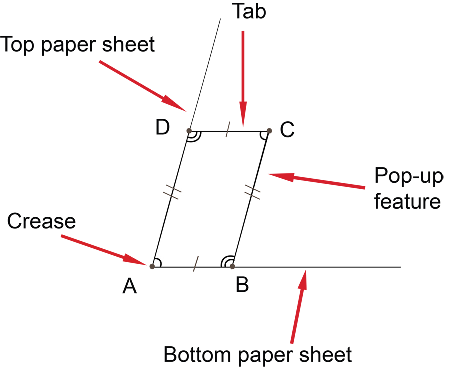
\includegraphics{figures/shared/01_Background/popup-diagram.pdf}
\caption{Cross-section of a popup card Figure modified from
https://en.wikipedia.org/wiki/File:Popup-diagram.svg.}
\end{figure}

The 90-degree popup card presents a tightly-constrained problem, with
opportunities for both interface design and algorithm innovations. We
present a system for designing popup cards, whose audience is
deliberately broad. We aim to make the pop=up card design process easier
and more fun.

Typically, users create popup cards through manual methods. For example,
a user might sketch out shape on a card in pencil, and then measure with
a rule to find locations to place folds. Or, they might \footnote{These
  are behaviors we observed by watching users create pop-up cards.}

\section{Motivation}\label{motivation}

\emph{This section is co-authored with Marissa Allen}

\begin{figure}[htbp]
\centering
\includegraphics{figures/shared/02_Overview/allcards.pdf}
\caption{A sample of cards created using Foldlings. For larger images
and fold patterns, see \nameref{appendix-d-sample-cards} on page
\pageref{appendix-d-sample-cards}.}
\end{figure}

We set out to create a tool that would help people design 3D pop-up
cards. We were driven by the desire to create original kirigami designs
without a template. As we progressed in our project, we began to focus
on developing a tool that would provide a way to create pop-ups more
intuitively, without explicitly understanding how to create a valid
90-degree pop-up card. Our tool allows users to design, iterate, and
preview an original pop-up card before they even pick up a pair of
scissors.

We outline some user stories --- potential use cases for our software:

\begin{itemize}
\itemsep1pt\parskip0pt\parsep0pt
\item
  George is an avid scrapbooker. He uses Foldlings to create small
  pop-up elements to liven up his scrapbooks. Sometimes he, creates
  cards to commemorate moments --- other times, he pastes photos or
  other media onto a pop-up card structure created with our app.
\item
  Sally designs cards for a commercial greeting card company. She uses
  Foldlings to create rough prototypes and concept sketches for pop-up
  cards. After getting feedback from the rest of her team, she brings
  the exported SVG file into Adobe Illustrator to refine the final card
  designs.
\item
  Jim forgot to make a card for his wife's anniversary present, and
  she's coming home in an hour! He downloads Foldlings from the Apple
  App Store, and is able to quickly design and create a beautiful card.
\item
  Alex is a creative college student who wants to continue making things
  for her friends and family. She wants to explore pop-up cards, but
  doesn't like any of the templates she's found online and can't pay for
  pop-up design books. She finds Foldlings in the Apple App Store and
  tests her creativity with our tool.
\item
  Kate, a middle school math teacher, is teaching a module on pop-up
  card geometry. She uses Foldlings to teach the students about the
  parallelogram constraints between planes as cards fold. By using our
  app, her students gain an intuitive understanding of the geometric
  constraints.
\end{itemize}

\section{Technical Overview}\label{technical-overview}

\emph{This section is co-authored with Marissa Allen}

Our algorithmic simulation and validity detection is based on a tight
set of constraints to the pop-up card problem. We require the card to
have a central main valley fold --- from there we can determine the
orientation of planes, as alternating folds fold in opposite
orientations. The card then folds 180 degrees; this implies
parallelogram constraints between all the edges in a sideways
cross-section (with the exception of v-fold features).

We capture touch input, translating touches into cuts and folds
depending on the geometry of the fold feature. We validate fold features
before they are added to the sketch, ensuring that the design can fold
in 3D. At this point, we also perform bezier path operations to modify
existing edges in the sketch based on the new design element. When a
fold feature is added to the sketch, we re-calculate planes (areas
enclosed by cuts and folds) by traversing a directed graph of edges in
the sketch. Based on these 2D planes, we create 3D planes, which are
oriented and translated based on their relationship to other planes in
the sketch. In 3D, we animate planes in response to user input. Each of
the planes is translated in relation to the plane oriented above the
fold and rotated in relation to the main driving joint.

Our approach constructs a tree representation of the planes based on
fold adjacency and uses this for determining the parent child
relationships in the simulated 3D view. We also use a tree-based
structure to store associations between logical geometric units.

\subsection{Development Process}\label{development-process}

\begin{figure}[htbp]
\centering
\includegraphics{figures/shared/02_Overview/gitflow.png}
\caption{Branches in our github.com repository.}
\end{figure}

We designed and developed the software interactively, frequently testing
prototypes with users. We used github to build Foldlings
collaboratively. Our workflow involved creating new code branches for
each feature, and reviewing the changes before merging back into the
master branch of the codebase. The full source for our software is
available at \url{http://github.com/harquail/foldlings/}.

\section{Pipeline Overview}\label{pipeline-overview}

\emph{This section is co-authored with Marissa Allen}

\begin{figure}[htbp]
\centering
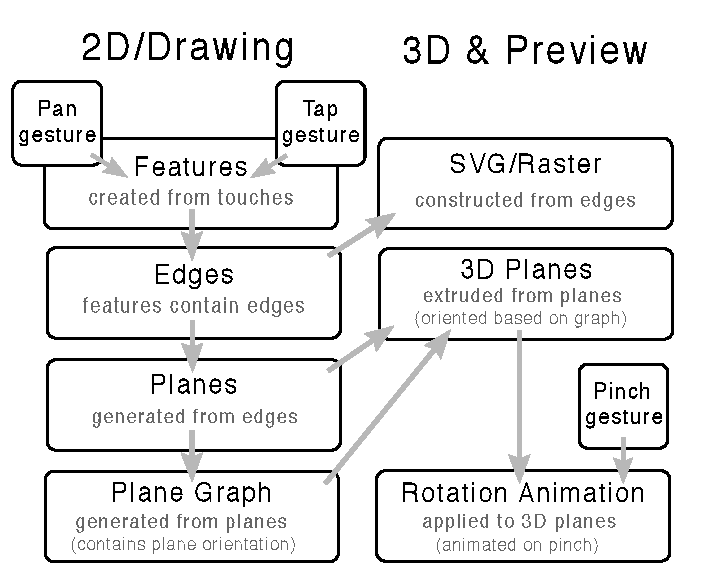
\includegraphics{figures/shared/02_Overview/pipeline.pdf}
\caption{Overview of data flow between 2D and 3D systems.}
\end{figure}

To begin, a user draws a design using the fold feature tools: box fold,
polygon, freeform and v-fold. These tools create a pattern of cuts and
folds, displaying an interactive preview of the design as the user
creates it. The cuts and folds created with these tools remain
associated with each other, and can be modified or deleted as a unit.

Each time a new shape is added to the design, it is evaluated for
validity: whether it can fold to 90 degrees and be parsed into
individual planes. The planes are then linked together in an acyclic
graph based on the planes' abutting top edges. This acyclic graph allows
us to shade planes based on orientation in 2D and simulate the design in
3D. Each feature can also be modified or deleted, by tapping on the
feature an selecting an entry from the list of available options.

This process continues until the user previews the design in 3D. The 3D
preview displays a simulation of how the design will fold, which can be
manipulated using a pinch gesture. The user is free to return to the 2D
drawing interface and continue editing his/her design or save the design
as either a raster file or SVG vector file. After this step, the user
can print and cut the raster file or open the SVG file on a laser cutter
or other cutting tool. We automatically save designs locally when
leaving the design workspace, so users can restore their work.

Figure 1.6 shows the full pipeline for designing cards. It shows a
user's design process, starting with concept sketches, and moving
through iterations of the sketch using the 3D preview to test the
design. Finally, the user exports the design as a fold pattern, and cuts
and folds the pop-up card.

\begin{figure}[htbp]
\centering
\includegraphics{figures/shared/02_Overview/sinewave.pdf}
\caption{A full outline of the design process for Foldlings, from
initial concept sketches to full realization of a paper pop-up card.}
\end{figure}

\section{Related Work}\label{related-work}

\textbf{\textgreater{}\textgreater{}TODO: Complete w/Marissa}

\emph{This section is co-authored with Marissa Allen}

Our approach to pop-up creation does not require glue or 3D modeling
experience, but is more similar to kirigami. Glue-based design presents
different affordances than kirigami, but requires an assembly stage that
disconnects the initial 2D pattern from the final pop-up geometry
{[}Glassner 1998{]}. Others approach the pop-up design problem from the
opposite direction: creating designs by modeling in 3D space {[}Ruiz et
al. 2014{]}. {[}Li et al. 2010{]} transform 3D models into paper
architectures that are stable and rigid. A drawback to this approach is
that it does not preserve the original model's features. Compared to
existing tools, Foldlings allows novice users more opportunities for
free-form, artistic expression in the pop-up medium.

There has been prior work done on automated methods to create a pop-up
schematic. For example, Li, Xian-Ying, et al. develop an algorithm that
transforms user-defined models into paper architectures that are stable
and rigid. Because their algorithm modifies the input geometry given by
the user, the end result does not preserve the original model's
features. Other attempts to create pop-up cards such as Abel, Zachary,
et al. --- can only take in simple polygonal meshes and require the user
to fold and glue additional pieces of paper together, whereas our
approach creates a pop-up card with arbitrary shapes from a single piece
of paper. These methods also impose strict constraints on user input,
which requires the end user to know how to model an object in 3D and
thus is not accessible to novice users.

Our approach to smoothing user input as the user draws his/her design is
similar to Johnson, Gabe, et al. After a user has drawn lines in their
program, they edit these lines depending on what mode the user is in and
the drawing is then sent to a laser-cutter. However, our method
automatically interpolates the lines given by the user and transforms
them into smoothed Bezier curves, ready to be printed.

Hendrix, Susan L., and Michael Eisenberg. ``Computer-assisted pop-up
design for children: computationally enriched paper engineering.''
Advanced Technology for Learning 3.2 (2006): 119-127.
\citet{hendrix2006computer}

The pop-up tool described by this paper is very similar to our current
design. However, this tool was built as an introduction to the
engineering sciences and not as a tool to aid artistic design. Perhaps
as a result of an engineering-centric design methodology, the pop-up
tool has a more restrictive UI than ours. Their program is designed to
only create the simple folding mechanism of the pop-up card. Adding
arbitrary cuts and multiple layers is not supported and must be added
later.

Okamura, Sosuke, and Takeo Igarashi. ``An interface for assisting the
design and production of pop-up card.'' Smart Graphics. Springer Berlin
Heidelberg, 2009. \citet{okamura2009interface}

This paper describes a program to design elaborate 180º pop-ups that can
be applied to both cards and books strictly within a 3d environment.
Their manufacturing process is additive, using glue to connect the
pieces. They implement collision testing and multiple components inside
their pop-up program. However, their program does not incorporate the
main folding piece in designing their pop-ups, it is simply a mechanical
driver for the rest of the design. Therefore, a user cannot design a
pop-up that consists of only one piece of paper that does not require
gluing.

Way, Der-Lor, Yong-Ning Hu, and Zen-Chung Shih. ``The Creation of V-fold
Animal Pop-Up Cards from 3D Models Using a Directed Acyclic
Graph.''Advances in Intelligent Systems and Applications-Volume 2.
Springer Berlin Heidelberg, 2013. 465-475. \citet{way2013creation}

The tool described in this paper creates pop-ups from 3d models. The
tool segments a 3d model and then uses shape recognition to create paper
models in pop-up cards. The authors create an acyclic graph from these
segments and use the nodes to drive a simulation of the pieces based on
opening and closing the card. This paper has a similar simulation
technique to our approach. However, they generate their designs from 3d
shapes instead of 2d patterns.

\chapter{Design}

\section{Design Philosophy}\label{design-philosophy}

Our design philosophy is simple: follow the user. As often as possible,
we presented our interface concepts to potential users, and allowed
their feedback to guide the design process through the final prototype.

Following a methodology roughly following agile methodologies, we
designed and developed the application collaboratively
(\citet{martin2003agile}). Our process was driven by user experience
design, rather than graphic design. That is, we spent relatively little
time polishing aesthetic interface details, and instead focussed on the
core interactions of the application.

\includegraphics{figures/30_UI_Design_Philosophy/gitflow.png}
\textbf{\textgreater{}\textgreater{}TODO: FIX}

mention affordances of iPad --- cite Gibson/teapot guy. We chose to
design for the iPad as a way of forcing the interface. With a simple,
gesture-based interface, we were forced to

Throughout the design process, we explored the conflict between
creativity and rigid geometric constraints. That is, interfaces that
give the user more room for creative generally tend to make it more
difficult to create designs that will fold correctly in 3D. We aimed for
an interface that provides a great deal of flexibility and creativity,
while guaranteeing that all popup card designs created with it are
valid. Two primary systems maintain this balance.

\begin{enumerate}
\def\labelenumi{\arabic{enumi})}
\itemsep1pt\parskip0pt\parsep0pt
\item
  Tool-based feature creation allows for complex geometry while solving
  geometric constraints transparently.
\item
  The validity system disallows geometry that would interfere with
  existing design elements.
\end{enumerate}

We strive to design an interface that is \textbf{modular},
\textbf{friendly}, and \textbf{delightful}. \textbf{Modularity} stems
from the conception of the pop-up card as a collection of discrete units
that can be acted on individually. Modularity allows users to think in
terms of shape constructions, without concern for individual cuts and
folds. Users can modify, add, and delete individual geometric units,
without modifying the majority of their design. \textbf{Friendliness} is
seen in the careful structuring of our experience to make getting
started as painless as possible. For example, we structure our tutorial
not as a step that must be completed before using the app, but as a
series of brief videos that appear when using a tool for the first time.
\textbf{Delight} comes from small, unexpected details that enhance the
user experience. For example, our color scheme for planes is inspired by
the colors of construction paper. Through this color scheme, we hope to
evoke the spirit of fun and exploration associated with casual
paper-craft.

\section{Interface Iteration}\label{interface-iteration}

\begin{quote}
\begin{quote}
TODO: figure showing alpha UI
\end{quote}
\end{quote}

discuss move from drawing cuts \& folds directly to templating

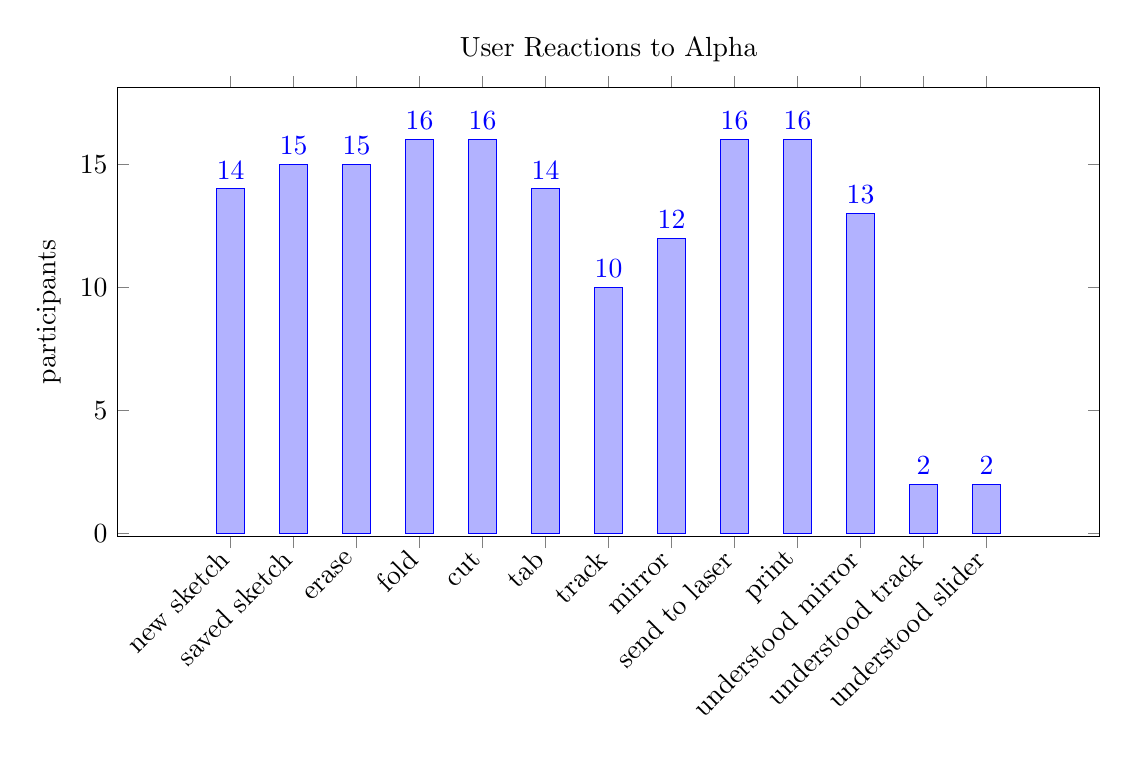
\begin{tikzpicture}
  \begin{axis}[
    title=User Reactions to Alpha,
    ybar,
    enlargelimits=0.15,
    x=0.8cm,
    legend style={at={(0.5,-0.2)},
      anchor=north,legend columns=-1},
    ylabel={participants},
    symbolic x coords={new sketch,saved sketch,erase,fold,cut,tab,track,mirror,send to laser,print,understood mirror,understood track,understood slider},
    xtick=data,
    nodes near coords, 
    nodes near coords align={vertical},
    x tick label style={rotate=45,anchor=east},
    ]
    \addplot coordinates {(new sketch,14)(saved sketch,15)(erase,15)(fold,16)(cut,16)(tab,14)(track,10)(mirror,12)(send to laser,16)(print,16)(understood mirror,13)(understood track,2)(understood slider,2)};
  \end{axis}
\end{tikzpicture}

\textbf{\textgreater{}\textgreater{}TODO: separate user comments from
observation}

\begin{longtable}[c]{@{}l@{}}
\caption{Feedback from first user test.}\tabularnewline
\toprule
\begin{minipage}[b]{0.82\columnwidth}\raggedright\strut
Comments
\strut\end{minipage}\tabularnewline
\midrule
\endfirsthead
\toprule
\begin{minipage}[b]{0.82\columnwidth}\raggedright\strut
Comments
\strut\end{minipage}\tabularnewline
\midrule
\endhead
\begin{minipage}[t]{0.82\columnwidth}\raggedright\strut
want option to fold other way, wanted to be able to draw over exising
line with tab tool, made a cake, crashed on returning to sketch
\strut\end{minipage}\tabularnewline
\begin{minipage}[t]{0.82\columnwidth}\raggedright\strut
track and slider will need explanation; wanted to use non-horizontal
folds
\strut\end{minipage}\tabularnewline
\begin{minipage}[t]{0.82\columnwidth}\raggedright\strut
wanted to fold by pinching, want to rename? delete, move them around?
\strut\end{minipage}\tabularnewline
\begin{minipage}[t]{0.82\columnwidth}\raggedright\strut
wanted ortho views, hold to view info about tool, examples. Interactive
tutorial
\strut\end{minipage}\tabularnewline
\begin{minipage}[t]{0.82\columnwidth}\raggedright\strut
erased master fold, crashing at preview step
\strut\end{minipage}\tabularnewline
\begin{minipage}[t]{0.82\columnwidth}\raggedright\strut
wanted interactive tutorials, made a cat
\strut\end{minipage}\tabularnewline
\begin{minipage}[t]{0.82\columnwidth}\raggedright\strut
momentary confusion getting back to sketch
\strut\end{minipage}\tabularnewline
\begin{minipage}[t]{0.82\columnwidth}\raggedright\strut
wanted to move around existing sketches
\strut\end{minipage}\tabularnewline
\begin{minipage}[t]{0.82\columnwidth}\raggedright\strut
confused about concept of a laser cutter
\strut\end{minipage}\tabularnewline
\begin{minipage}[t]{0.82\columnwidth}\raggedright\strut
wanted interative tutorial
\strut\end{minipage}\tabularnewline
\begin{minipage}[t]{0.82\columnwidth}\raggedright\strut
wanted to fold 3d preview by hand
\strut\end{minipage}\tabularnewline
\begin{minipage}[t]{0.82\columnwidth}\raggedright\strut
very frustrated by tools that aren't implemented yet
\strut\end{minipage}\tabularnewline
\begin{minipage}[t]{0.82\columnwidth}\raggedright\strut
confused by track \& slider
\strut\end{minipage}\tabularnewline
\begin{minipage}[t]{0.82\columnwidth}\raggedright\strut
needed heavy guidance; completely confused by track/slider
\strut\end{minipage}\tabularnewline
\begin{minipage}[t]{0.82\columnwidth}\raggedright\strut
wanted more snapping/guidance on creating valid designs
\strut\end{minipage}\tabularnewline
\begin{minipage}[t]{0.82\columnwidth}\raggedright\strut
fairly self-sufficient after tools were explained, made a house, moved
slowly, waiting for planes to calculate
\strut\end{minipage}\tabularnewline
\bottomrule
\end{longtable}

\section{Interactions}\label{interactions}

Through the iterations described in the previous chapter, we arrived at
Foldlings' tool-based system for card design.

\subsection{Tap Options}\label{tap-options}

describe tap options

\textbf{\textgreater{}\textgreater{}TODO: add figure showing tap
options}

\subsection{Tool Interactions}\label{tool-interactions}

Some interactions are common to all features. To add a feature, you
select the tool that creates features of that type. Each feature
type\footnote{(Except for the master card)} has a corresponding button
in the toolbar at the bottom of the sketches. In general, all features
are defined by dragging in the drawing area. Features are generally
completed by releasing the drag. As long as you remain in that tool, you
can continue creating features of that type by dragging. Having
consistent tool interactions helps reduce the burden of learning new
tools, and allows for a scaffolded user experience.
\textbf{\textgreater{}\textgreater{}TODO cite scaffolding lit}

\textbf{\textgreater{}\textgreater{}TODO: add tap options, how to draw,
and a description of the tool-based interface in general}

\subsubsection{Box Fold}\label{box-fold}

A box fold is created by dragging.

\subsubsection{FreeForm}\label{freeform}

Drag, then truncate

\subsubsection{Polygon}\label{polygon}

Tap to add points or drag Special case, tap within poly with poly tool
selected doesn't add points

\subsubsection{V-Fold}\label{v-fold}

two-step feature vertical cut, then drag on driving fold

\subsection{Tutorial}\label{tutorial}

We eschewed detailed drawing instructions or a separate tutorial mode,
in favor of short video tutorials that appear the first time each tool
is used. These tutorials can also be accessed by tapping the feature
icons on the about page.

\begin{figure}[htbp]
\centering
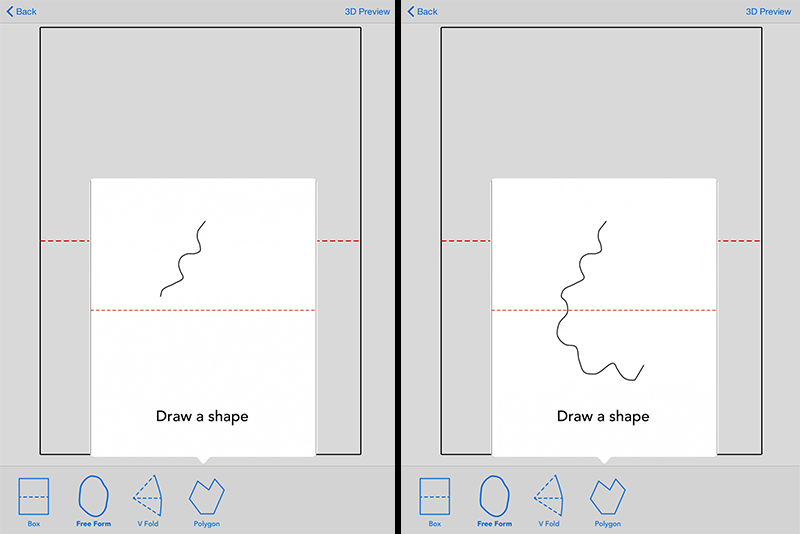
\includegraphics{figures/32_UI_Tool_Interactions/tutorial_step_one_two.png}
\caption{Free-form shape tutorial video.}
\end{figure}

We also show helpful tips between screens --- for example, when moving
to 3D preview and restoring from a saved sketch.

\subsection{Warnings and Errors}\label{warnings-and-errors}

We display warnings and errors as bright-red banners at the top of the
sketch view when. These warnings are displayed in response to failing
the validity checks performed when adding a feature to the sketch.

\begin{figure}[htbp]
\centering
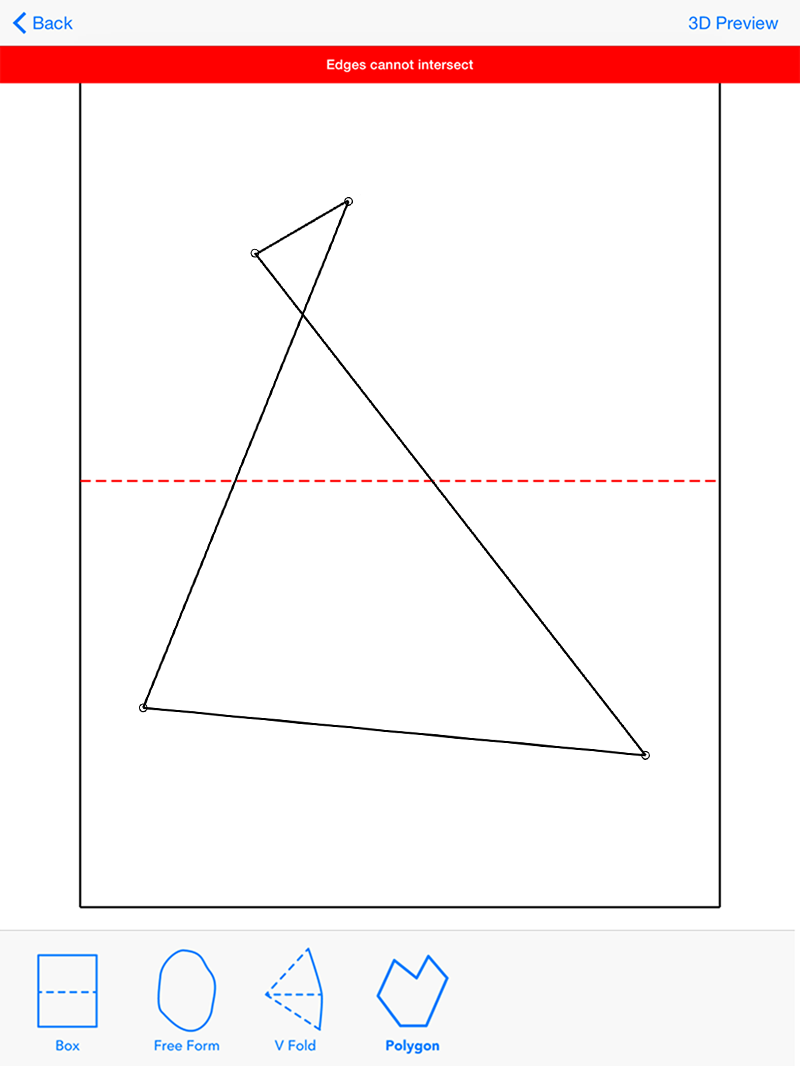
\includegraphics{figures/32_UI_Tool_Interactions/error_message.png}
\caption{An error message shown when rejecting a polygon with
intersecting edges.}
\end{figure}

The goal of these warnings is to give users descriptive feedback when
errors occur, and to give them an intuitive sense of which actions
create invalid features.

\subsection{Send to Laser Cutter}\label{send-to-laser-cutter}

In the three-dimensional preview, users can tap the ``send to laser
cutter'' option. This feature sends the user an email with an attached
SVG file. This file can be fed to a laser cutter or paper cutting
machine, or can be opened in a vector graphics program to make further
changes.

\subsection{Print}\label{print}

In addition to sharing an SVG file for laser cutting, users can press
``share''. This version is essentially screenshot of the 2D sketch, and
can be printed, emailed, or shared via social media. Typically, this is
the option a user would choose to cut and fold their design by hand.

\begin{figure}[htbp]
\centering
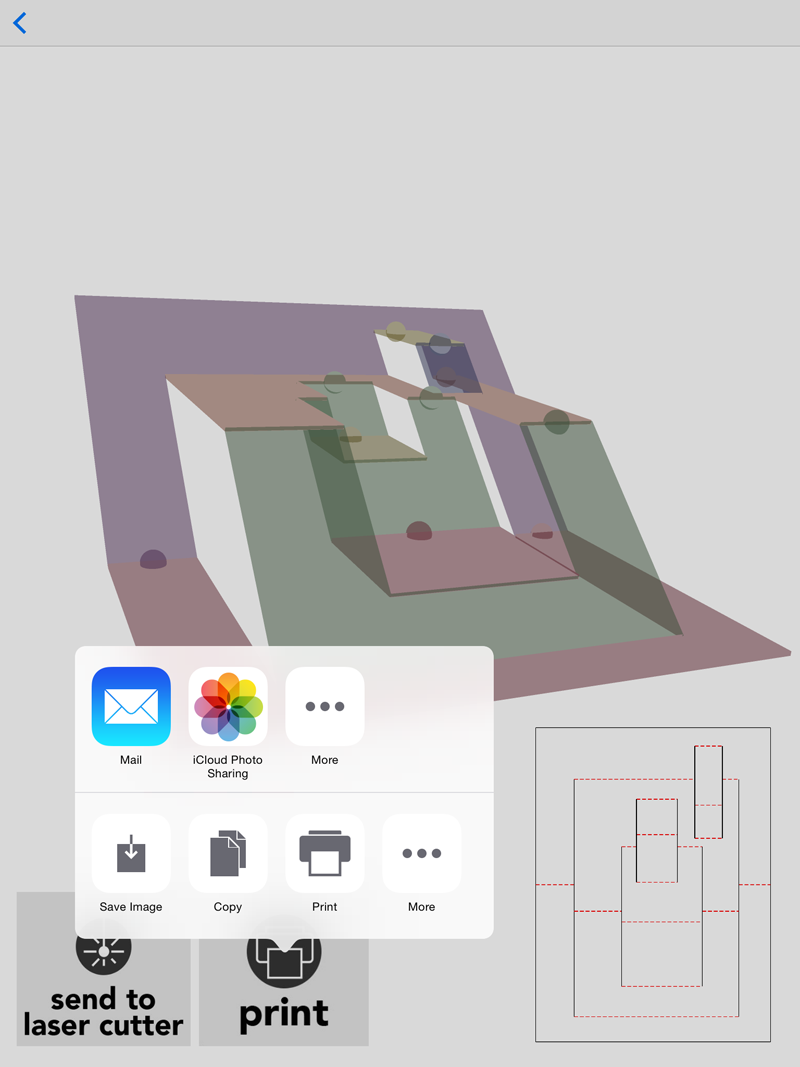
\includegraphics{figures/32_UI_Tool_Interactions/3d-share.png}
\caption{Options for sharing a fold pattern from the 3D preview.}
\end{figure}

\section{Interface Data Structures}\label{interface-data-structures}

We will refer to several data structures throughout the discussion of
user interface design and implementation. These are the primary means of
storing user input processed by the tools, and are processed by our
algorithms to draw designs in 2D and simulate them 3D\footnote{This
  section only describes the primary data structures necessary for
  constructing fold and patterns from user input, detecting planes, and
  determining the relationships between, not the systems for drawing
  features in 2D or 3D. For a discussion of 2D drawing, see sections.
  For a discussion of, see .
  \textbf{\textgreater{}\textgreater{}TODO:cite marissa
  \textgreater{}\textgreater{}TODO reference section}}.

\subsection{Edges}\label{edges}

\begin{figure}[htbp]
\centering
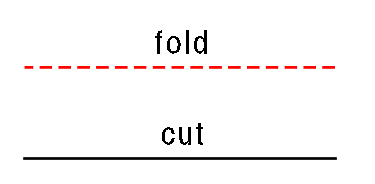
\includegraphics{figures/33_UI_Interface_Data_Structures/foldvsedge.pdf}
\caption{In Foldlings, cuts are displayed as solid black lines. Folds
are displayed as dotted red lines. This convention is familiar to those
who use traditional instructional books
(\citet{berenson1972kirigami},3).}
\end{figure}

An Edge represents a cut or fold. Edges are the basic building block of
planes, and an integral element of all fold features. An edge is
minimally defined by a start point, end point, and a a type (either cut
or fold). This minimal definition represents a straight edge between two
points. In addition, an Edge can contain further information: the bezier
path drawn to create it (for non-straight edges), and a reference to the
plane or feature it is a part of. Additionally, each edge contains a
reference to its ``twin'' edge.

\subsubsection{Twin Edges}\label{twin-edges}

Although it is often simplest to think of edges as cuts and folds
created by the user, the reality in Foldlings is slightly more
complicated. For each edge that the user creates using a tool, two edges
are created. We create edges with direction, such that there is an edge
from the start point to the end point of the edge, and another edge
starts at the endpoint and has the reverse path of the original edge.
This distinction is most important when detecting planes from
edges\footnote{\textbf{\textgreater{}\textgreater{}TODO cite marissa's
  planes}}, but must also be taken into account whenever edges are
processed. For example, when drawing the 2D view of a sketch, we skip
drawing the twins of edges already drawn, which reduces drawing work by
half.

\begin{figure}[htbp]
\centering
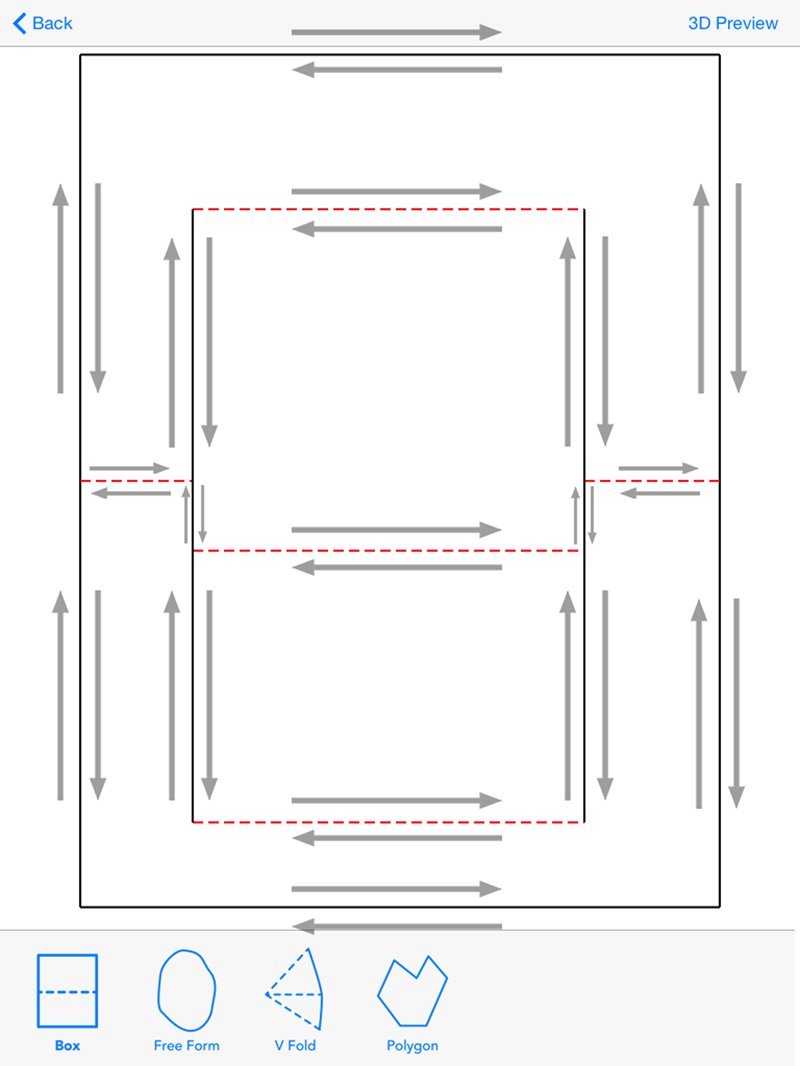
\includegraphics{figures/33_UI_Interface_Data_Structures/boxfold_34_edges.png}
\caption{This sketch contains 34 edges, with orientations shown by the
overlaid gray arrows.}
\end{figure}

\subsubsection{Driving Folds}\label{driving-folds}

\begin{figure}[htbp]
\centering
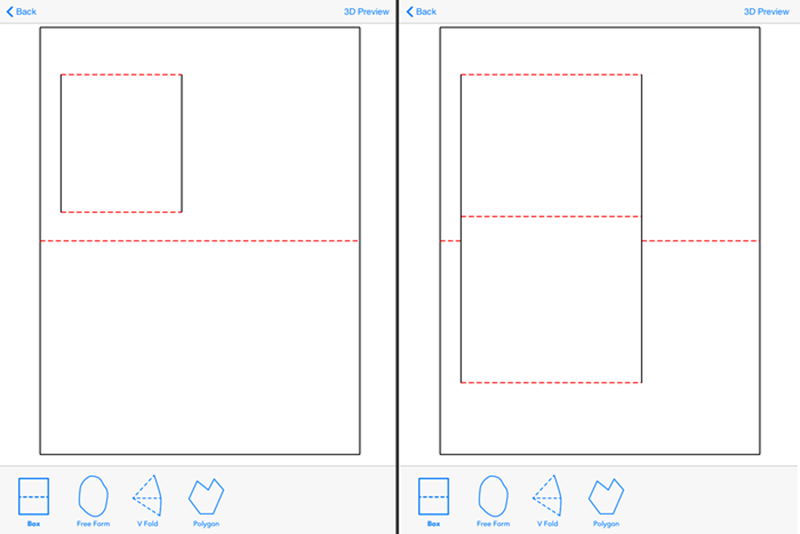
\includegraphics{figures/33_UI_Interface_Data_Structures/boxfold_driving_non_driving.png}
\caption{Left: a box fold mid-drag. The feature does not have a driving
fold. Right: a box-fold after the user has released the touch. The
feature's driving fold is the master card's middle horizontal fold.}
\end{figure}

A driving fold is not a special type of edge, but rather a relationship
between an edge in one feature and a feature ``spanning'' that edge. A
feature is said to span a fold when it is drawn on top of an existing
fold, so that it has horizontal folds on both sides of the middle fold.

An edge can be the driving fold for more than one feature, but each
feature has only one driving fold (if there are multiple potential
driving edges at the same height, the leftmost edge is selected. The
driving fold is important for calculating parent-child relationships
between features: a feature's parent is the feature that contains it's
driving fold\footnote{The exception to this rule is holes ---~a hole's
  parent is the feature that contains it.}. These parent-child
relationships are described in more detail in the
\nameref{nested-features} section on page \pageref{nested-features}.

\subsubsection{Fold Orientation}\label{fold-orientation}

\begin{figure}[htbp]
\centering
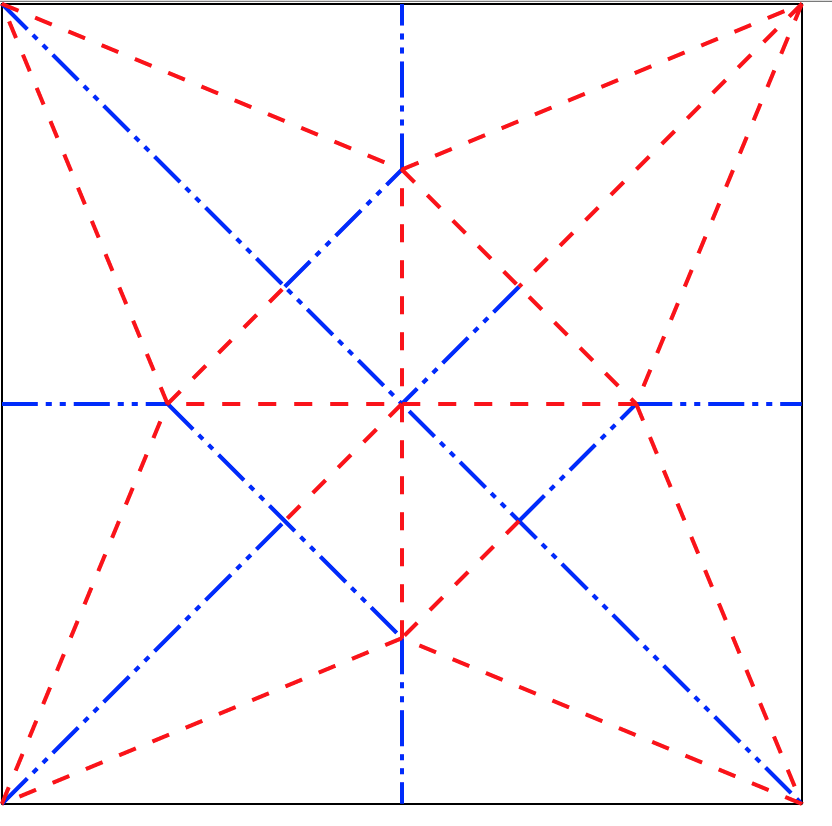
\includegraphics{figures/33_UI_Interface_Data_Structures/maekawas-theorem.png}
\caption{Kirigami fold pattern (\citet{maekawas-theorem}).}
\end{figure}

Traditionally, kirigami patterns indicate direction for folds:
``mountain/hill'' or ``valley''. These folds form angles in opposite
directions ---~mountain folds are pinched away from the paper surface,
while valley folds are pinched into the surface. In Foldlings, edge
orientations are determined by iterating through the plane tree
structure described in \textbf{\textgreater{}\textgreater{}TODO: CITE
MARISSA HERE}.

\subsection{Planes}\label{planes}

Planes are an enclosed shape, bounded by edges. Plane are detected from
edges by traversing the directed edge graph, as described in
\textbf{\textgreater{}\textgreater{}TODO: CITE MARISSA HERE}. They are
drawn as colored areas in the two-dimensional sketch, and simulated in
the 3D preview as shapes that rotate about a pivot point. In order to
simulate the planes in 3D, we construct parent-child relationships
between the planes, which determine how they move during simulation.

\begin{figure}[htbp]
\centering
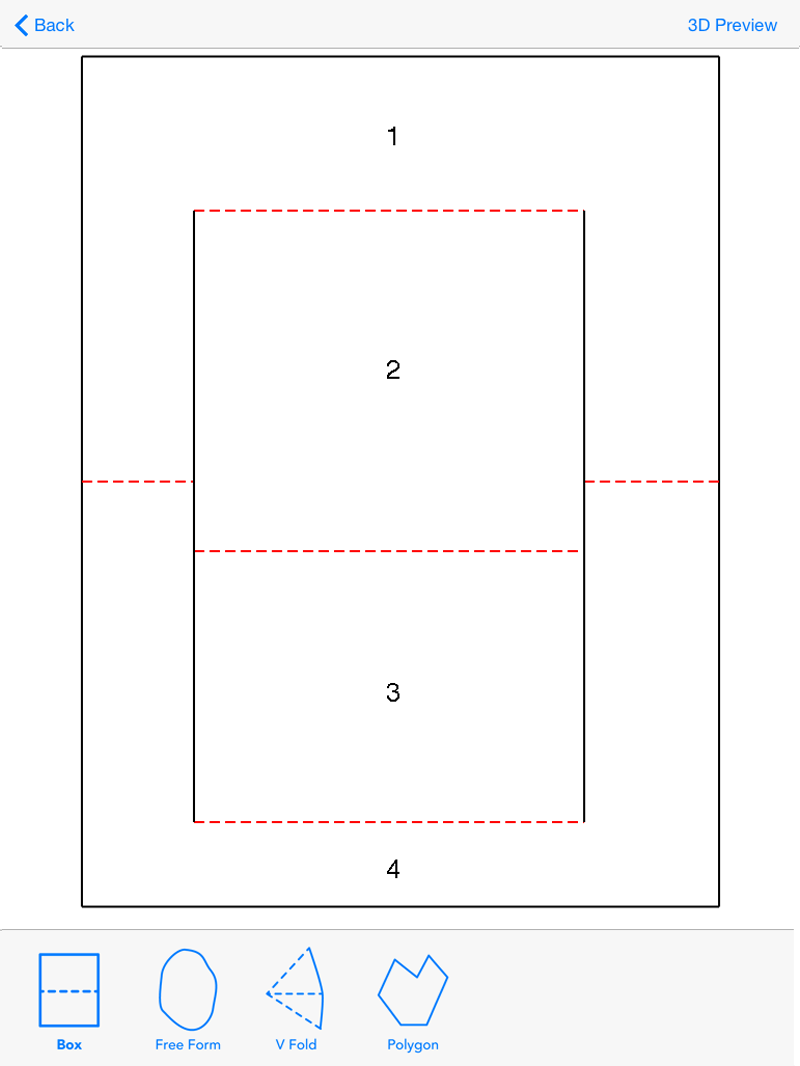
\includegraphics{figures/33_UI_Interface_Data_Structures/boxfold_planes.png}
\caption{Planes in a simple sketch, numbered by ancestry. Starting at
the root plane 1, each successive plane is the child of the previous
numbered plane.}
\end{figure}

\begin{figure}[htbp]
\centering
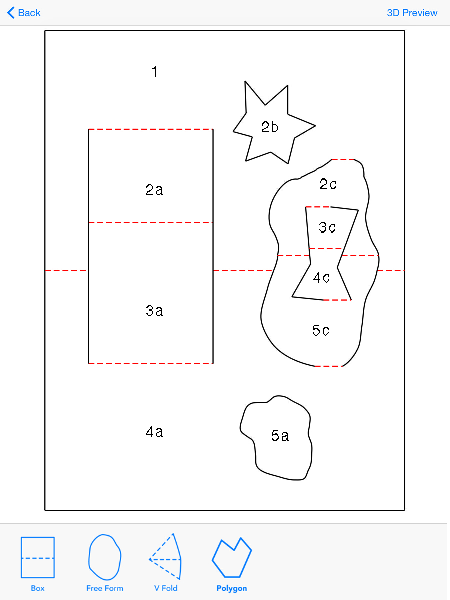
\includegraphics{figures/33_UI_Interface_Data_Structures/complex_sketch.pdf}
\caption{Planes in a more complex sketch, numbered by ancestry. Starting
at the root plane 1, each successive plane is the child of the previous
numbered plane. Letters indicate branches within the plane tree (I.e. 3a
is the child of 2a.}
\end{figure}

\subsection{Fold Features}\label{fold-features}

The central data structure of Foldlings is the FoldFeature: a
representation of a shape drawn by the user that folds in 3d. Each fold
feature is a single design element ---~and can be individually created,
modified, and deleted. There are five classes of FoldFeature:
MasterCard, BoxFold, FreeForm, Polygon, and V-Fold, representing
differences in drawing behavior, geometry, and (the differences are
described in detail below). Each of these features is a subclass of the
FoldFeature superclass.

All FoldFeatures have functionality in common:

\begin{itemize}
\itemsep1pt\parskip0pt\parsep0pt
\item
  Each feature contains a list of edges in the feature ---~cuts and
  folds, including twins.
\item
  Each feature has a driving fold --- in the case of unconnected
  features, such as the master card and holes, the driving fold is nil.
\item
  Each feature can be deleted from the Sketch, ``healing'' the sketch by
  closing gaps left in any
\item
  Features implement the encodeWithCoder and decodeWithCoder methods,
  allowing them to be serialized to a file on the device and restored
  from the saved file.
\item
  Each feature can provide a list of current ``tap options'' --- actions
  that can be performed on the feature given its state.
  \textbf{\textgreater{}\textgreater{}TODO:SEE tap options in interface
  design}
\item
  Each feature can perform hit-testing: given a point, it can determine
  whether that point is inside or outside the feature.
\end{itemize}

\subsubsection{Master Card}\label{master-card}

Each sketch always contains a single master feature, which is the
ancestor of all other features. It is a simplification of the box fold,
in that it contains three horizontal folds with connecting vertical
cuts. Users do not create features of this type~--- each sketch begins
with one. All of the edges in the master feature are marked with a flag
indicating that they belong to the master feature, because master
feature edges and planes are sometimes treated differently than normal
edges. For example, the parent-child relationships between planes are
constructed by starting at the top plane in the master feature,
determined by edge type and height.

\begin{figure}[htbp]
\centering
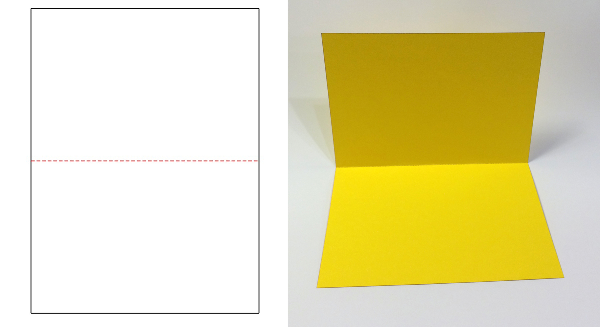
\includegraphics{figures/33_UI_Interface_Data_Structures/mastercard.pdf}
\caption{Left: fold \& cut pattern of the master feature. Right:
laser-cut model of the same.}
\end{figure}

\subsubsection{Box Fold}\label{box-fold}

A box fold consists entirely of straight edges, and can be constructed
from two points: the top left point, and the bottom right. The middle
fold position is determined by the position of the driving fold. Box
folds are only valid if they have a driving fold.

\begin{figure}[htbp]
\centering
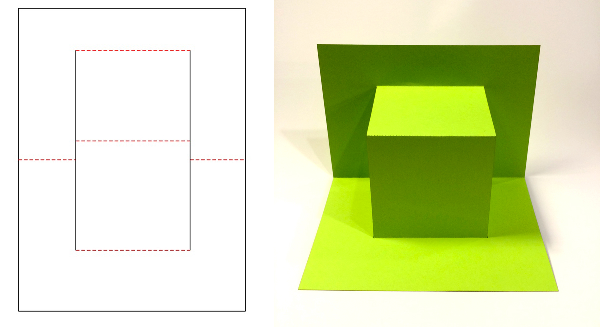
\includegraphics{figures/33_UI_Interface_Data_Structures/box.pdf}
\caption{Left: fold \& cut pattern of the master feature. Right:
laser-cut model of the same.}
\end{figure}

\subsubsection{Free Form}\label{free-form}

Free-form shapes are defined by a single, closed path. When the feature
is completed (by releasing the touch), the shape is truncated,
horizontal folds are added, and the path is split into multiple edges
(assuming the shape spanned a fold)\footnote{\textbf{\textgreater{}\textgreater{}TODO:SEE
  SECTION}}. The curved path is defined by a set of ``interpolation
points'' ---~points captured by sampling touch positions while a user
draws a shape on the screen. A bezier path is interpolated between these
points using the Catmull-Rom algorithm \textbf{TODO: CITE}.

Holes are a special case of FreeForm shapes, and are cut out from the
final design, rather than simulated as a separate plane. FreeForm shapes
that do not cross a fold are considered holes ---~drawn in white in the
2d sketch and drawn as subtractions from planes in the 3d view.

\begin{figure}[htbp]
\centering
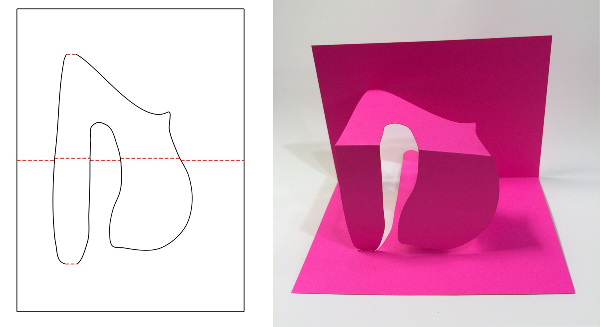
\includegraphics{figures/33_UI_Interface_Data_Structures/free.pdf}
\caption{Left: fold \& cut pattern of a freeform feature. Right:
laser-cut model of the same.}
\end{figure}

\subsubsection{Polygon}\label{polygon}

Polygons are created from a list of ``tap points'' constructed from user
input. As in free-form shapes, these points are connected with a bezier
path, and are truncated if they contain a driving fold when they are
completed. For polygons, this path consists only of straight line
segments. Unlike interpolation points, tap points can be moved at any
time during the drawing process.

Like FreeForm shapes, Polygons that do not have a driving fold are
considered holes.

\begin{figure}[htbp]
\centering
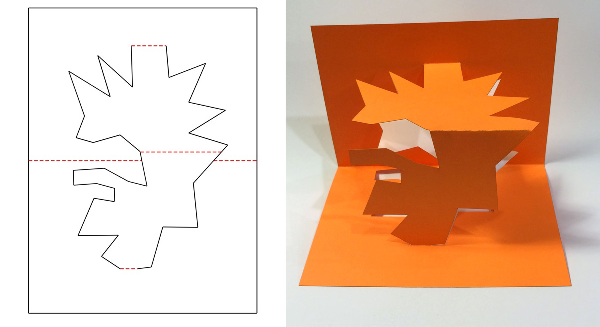
\includegraphics{figures/33_UI_Interface_Data_Structures/poly.pdf}
\caption{Left: fold \& cut pattern of a polygon feature. Right:
laser-cut model of the same.}
\end{figure}

\subsubsection{V-Fold}\label{v-fold}

\begin{figure}[htbp]
\centering
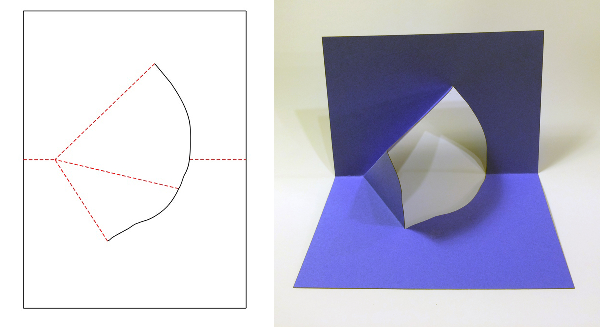
\includegraphics{figures/33_UI_Interface_Data_Structures/v.pdf}
\caption{Left: fold \& cut pattern of a v-fold feature. Right: laser-cut
model of the same.}
\end{figure}

V-Folds are defined by a path that crosses the driving fold, called a
``vertical cut.'' This path can be an arbitrary shape that crosses the
driving fold once. They are fully-defined by adding a point on the
driving fold. From this point, we construct three diagonal folds, two to
the top and bottom of the vertical cut, and one to a point that
intersects with the vertical cut at a point calculated to make a valid
90-degree feature.

\begin{figure}[htbp]
\centering
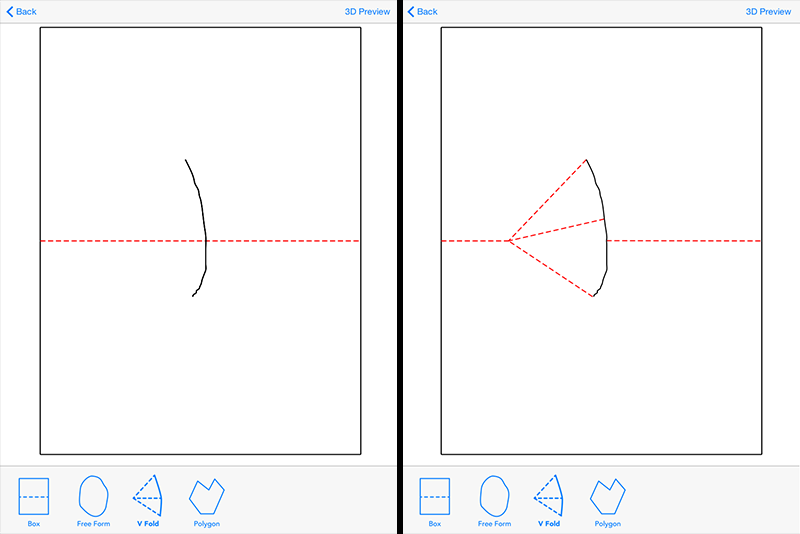
\includegraphics{figures/33_UI_Interface_Data_Structures/vfold_before_after.png}
\caption{Left: an unfinished v-fold, consisting only of a vertical cut.
Right: a v-fold after defining the point on the driving fold to create
diagonal cuts.}
\end{figure}

V-folds are only valid if they have a driving fold, and their vertical
cut intersects the driving fold exactly once.

\subsubsection{Hierarchy}\label{hierarchy}

Fold features have two types of hierarchy. The first is feature
hierarchy: each feature can have other features as children. When a
feature is drawn spanning a fold, its driving fold is set as the fold it
spans, and its parent is the feature that contains this driving fold.
Feature hierarchy allows us to consider each feature individually or as
a chain of features. For actions that only affect a single feature, we
need only consider the edges in the feature and it's driving fold. We
can also traverse the tree to perform actions on a chain of features.
The second type of hierarchy is parent-child relationships between
planes. Each plane has one or more children, forming a branching tree
that starts at the top plane of the master card and ends with the master
card's bottom plane as one of its leaf nodes. This hierarchy is
described in \textbf{\textgreater{}\textgreater{}TODO}, and is most
important for rendering the scene in 3D.

\subsection{Sketches}\label{sketches}

A sketch is the representation of the user's drawing ---~its primary
role is as a collection of features. It also contains information about
the current drawing state, and the state of user interaction (for
example, which features are currently being modified, and which tool is
selected).

\section{Saving}\label{saving}

Every time users leave a sketch, Foldlings archives the sketch to a
file, which can then be restored. Users restore a sketch by tapping on
one of the cards on the main screen. These cards can be deleted through
a long press on the sketch, which presents an option to remove the saved
file. This convention is familiar to iOS users.

\begin{figure}[htbp]
\centering
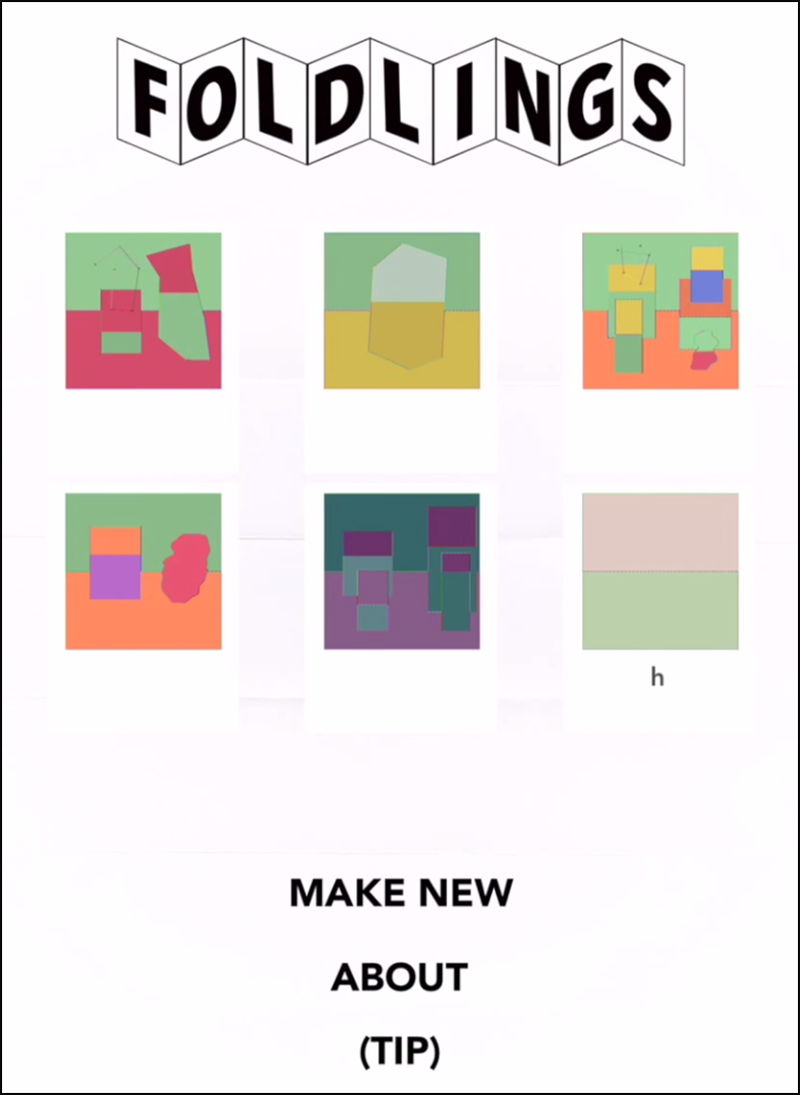
\includegraphics{figures/34_UI_Saving/saved_sketches.png}
\caption{Saved sketches displayed on the main screen.}
\end{figure}

In addition, we also save fold patterns for user designs to Amazon S3.
Saving these files allows us to debug user problems remotely and see the
kinds of cards users attempt to make with our software. Along with user
testing, these captured sketches have been instrumental to our design
process.

\chapter{Algorithms and Implementation}

\section{Interface Implementation}\label{interface-implementation}

One of the core components of Foldlings is the interface. To create
features, we capture touch input, display a preview of fold features as
the user creates them, and add created features to the fold pattern.
This system is outlined in Figure \ref{mvc}.

\begin{figure}[htbp]
\centering
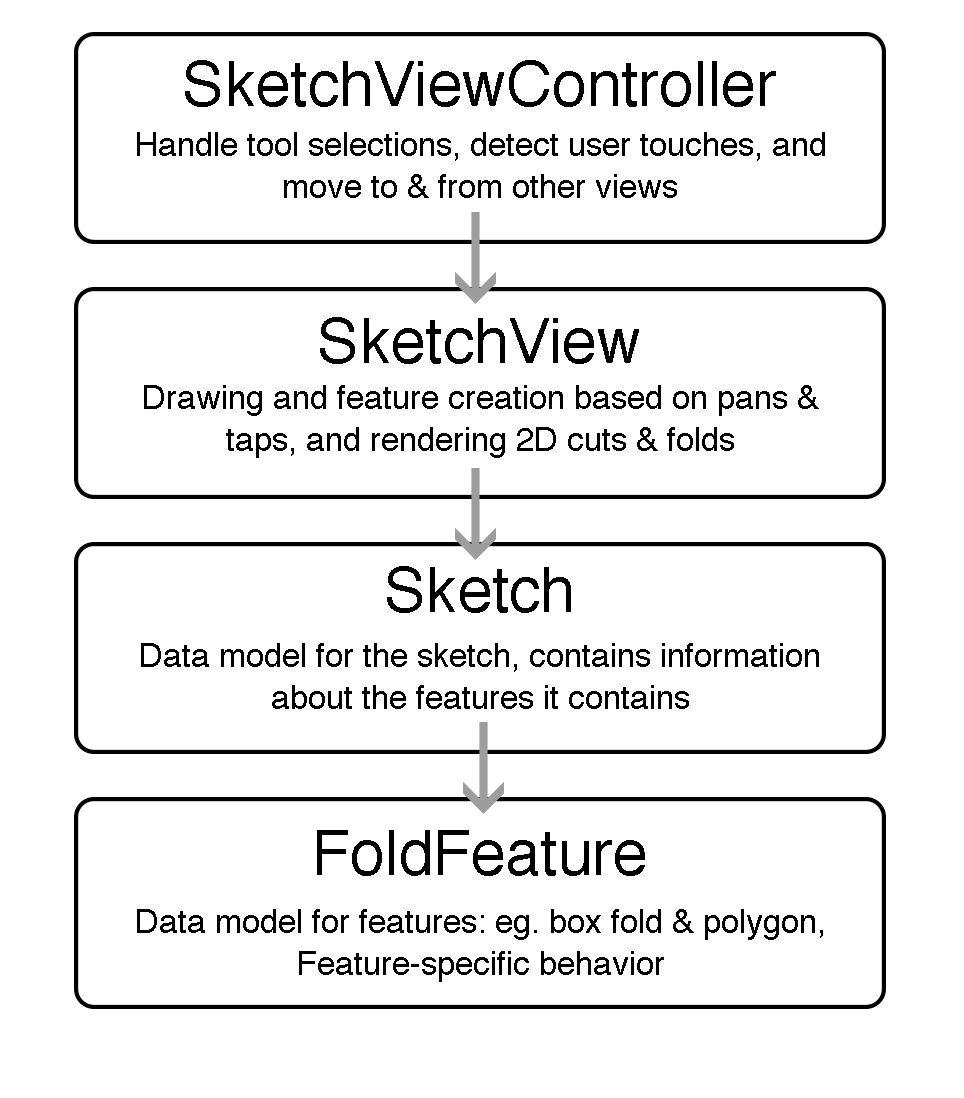
\includegraphics{figures/40_Tech_Interface_Implementation/sketchview-descendents-thesis-figure.png}
\caption{Relationship between interface classes: a SketchViewController
manages a SketchView that contains a Sketch that contains FoldFeatures.
\label{mvc}}
\end{figure}

Although this structure borrows heavily from the Model-View-Controller
design pattern, we do not follow the pattern strictly. The MVC paradigm
often becomes muddy, with much information shared between the separate
modules (\citet{veit2003model}). In our case, we separate modules not
purely based on MVC encapsulation but based on functionality. For
example, rather that strictly separating all touch handling into the
view controller or all drawing into the view, these responsibilities are
shared between the classes as needed to perform their roles. See section
\ref{touch-handling}, below, for more information.

\subsection{Touch Handling}\label{touch-handling}

In order to create features, we first need to capture touch input.
Foldings handles two types of touches: pan gestures, and tap gestures.
Apple describes gesture recognizers in the documentation for the
\emph{UIGestureRecognizer} class:

\begin{quote}
Gesture recognizers convert low-level event handling code into
higher-level actions. They are objects that you attach to a view, which
allows the view to respond to actions the way a control does. Gesture
recognizers interpret touches to determine whether they correspond to a
specific gesture, such as a swipe, pinch, or rotation. If they recognize
their assigned gesture, they send an action message to a target object.
The target object is typically the view's view controller, which
responds to the gesture\ldots{}
\end{quote}

In Foldlings, all gestures are captured by the SketchViewController,
which passes un-handled gestures on to classes lower down the chain. In
general, all taps are handled at the SketchViewController level; the
only exception to this rule is the Polygon feature, described in section
on page. \textbf{\textgreater{}\textgreater{}TODO PAGES}

\subsection{Tool Selection}\label{tool-selection}

Tool state is maintained by the SketchViewController. The
SketchViewController handles taps on tool buttons and features, and
passes pan gestures to the SketchView. The method called on the
SketchView depends on what feature was selected. The function below in
SketchView captures pan gestures, and calls the appropriate function
depending on the tool selected and the drawing state.

\small
\singlespacing 

\begin{pygmented}{swift}
    func handlePan(sender: AnyObject) {
        if(sketch.tappedFeature != nil){
            switch(sketch.tappedFeature!.activeOption!){
            case .MoveFolds:
                handleMoveFoldPan(sender)
            default: break
            }
        }
        else{
            switch (sketchMode) {
            case .BoxFold:
                handleBoxFoldPan(sender)
            case .FreeForm:
                handleFreeFormPan(sender)
            case .VFold:
                handleVFoldPan(sender)
            case .Polygon:
                handlePolygonPan(sender)
            default:
                break
            }
        }
    }
\end{pygmented}

\doublespacing
\normalsize

Within the specific function in SketchView, pan gestures are converted
into feature edges by listening to \emph{touchesBegan},
\emph{touchesMoved}, and \emph{touchesEnded}. When a pan begins, we
create a new feature of the appropriate type and set it as the currently
active drawing feature. When the pan is updated, we add and/or modify
edges in the active feature. When the pan ends, we make final
modifications to edges, validate the feature, and add it to the sketch.

Of course, the implementation of pan delegate methods varies widely
between features. For example, a diagonal pan with the box fold tool
selected would create folds and cuts to form a box between the start and
end point, whereas the same touch in the freeform tool would create

\subsection{Fold Feature Preview}\label{fold-feature-preview}

While the user is drawing, the SketchView displays a preview of the
feature in progress, to give feedback on the drawing. Meanwhile, the
SketchView also displays the previously drawn features that have been
added to the sketch. Although the display of cuts and folds for the
current feature is visually similar to those of the final feature, the
method of drawing a preview version of the currently active feature
varies from the generation of final feature edges.

We store the currently active feature separately, it is not added to the
list of features until it is completed and passes validation. Thus, its
edges are drawn by the function that draws all edges currently in the
sketch. For performance reasons, we display a preview of the active
feature on top of all features in the sketch --- modifications to
existing features, and expensive operations such as truncation for
freeform shapes, are performed only when the feature is added to the
sketch. During drawing, we display the set of preview edges stored in
the feature, which sometimes differ from the final feature edges.

For box folds, we display a preview of all the edges, but do not occlude
the middle fold until the feature is completed. For freeform features,
we do not perform truncation until the feature is completed (and spans a
driving fold). As a preview, the SketchView shows the user's touch path
as a cut. For polygons, we display control circles at vertices. These
circles indicate that the vertices are draggable, modifying edge
endpoints dynamically. For v-folds, we display a dynamic preview of the
vertical cut and top and bottom diagonal folds. The middle diagonal
angle is not calculated until the feature is added to the sketch.

\subsection{Feature Creation}\label{feature-creation}

Once the user completes a feature, we add it to the sketch\footnote{Assuming
  the feature is valid. See section on page
  \textbf{\textgreater{}\textgreater{}TODO: cite validity}}. Adding a
feature to the sketch requires modifying existing features in the
sketch, constructing parent-child relationships, and recalculating
planes from edges. How these tasks are achieved depends on the specific
FoldFeature class.

The specific implementations of the FoldFeature superclass are described
in Chapter \ref{tool-implementation} on page
\pageref{tool-implementation}. The Sketch class contains methods for
adding and removing features from the sketch. It also contains
lower-level functions for adding, removing, and replacing edges. These
methods are typically called by feature-specific methods that modify the
sketch, such as \emph{splitFoldByOcclusion}.

In addition to adding a feature to the sketch, we also calculate the
planes, as described in \textbf{\textgreater{}\textgreater{}MARISSA}.
This allows us to shade planes based on orientation. After calculating
planes from edges, relationships between planes are stored in the plane
tree within the sketch. Within \emph{getPlanes}, plane orientations are
set by traversing the plane tree, alternating between vertical and
horizontal.

\subsection{Hierarchy}\label{hierarchy}

Fold features have two types of hierarchy. The first is . Within each
feature,

A key aspect of blah blah blah is hierarchy

Features contain other features

both feature and plane hierarchy

\section{Tool Implementation}\label{tool-implementation}

Below is the definition of the FoldFeature superclass --- all features
created using Foldlings can override these methods to provide specific
functionality. For further discussion of the FoldFeature data structure,
see \textbf{\textgreater{}\textgreater{}TODO cite}.

\singlespacing 

\begin{pygmented}{swift}
var horizontalFolds:[Edge] = [] //list of horizontal folds
var featureEdges:[Edge]?        //edges in a feature
var children:[FoldFeature] = [] // children of feature
var drivingFold:Edge? // driving fold of feature
var parent:FoldFeature? // parent of feature
var startPoint:CGPoint?
var endPoint:CGPoint? // start and end touch points

/// splits an edge around the current feature
func splitFoldByOcclusion(edge:Edge) -> [Edge]
{
//by default, return edge whole
return [edge]
}
/// features are leaves if they don't have children
func isLeaf() -> Bool
{
return children.count == 0
}
/// options or modifications that can be made to the current feature
func tapOptions() -> [FeatureOption]?
{
  return [FeatureOption.PrintPlanes, FeatureOption.PrintEdges,
  FeatureOption.ColorPlaneEdges, FeatureOption.PrintSinglePlane]
}
/// whether a feature is drawn over a fold, determines whether 
/// a fold can be the driving fold for a feature
  func featureSpansFold(fold:Edge)->Bool
{
  return false
}
/// returns and calculates planes in a feature
func getFeaturePlanes()-> [Plane]{
  return featurePlanes
}
/// whether a feature contains a point
/// needs to be overridden by subclasses
func containsPoint(point:CGPoint) -> Bool{
  return self.boundingBox()?.contains(point) ?? false
}
\end{pygmented}

\doublespacing

\subsection{Box Fold}\label{box-fold}

talk about fold heights talk about occlusion

\subsubsection{FreeForm}\label{freeform}

talk about truncation talk about splitting

\begin{algorithm}[H]
 \KwData{this text}
 \KwResult{how to write algorithm with \LaTeX2e }
 initialization\;
 \While{not at end of this document}{
  read current\;
  \eIf{understand}{
   go to next section\;
   current section becomes this one\;
   }{
   go back to the beginning of current section\;
  }
 }
 \caption{Path Splitting}
\end{algorithm}

\subsubsection{Polygon}\label{polygon}

contrast with free-form talk about point dragging talk about truncation

\subsubsection{V-Fold}\label{v-fold}

talk about angle calculation

\section{Intersections Between
Features}\label{intersections-between-features}

As we observed at the Digital Arts Exhibition \footnote{see}, users
often. As a result, we implemented

\section{Validity}\label{validity}

One of the primary goals of our software is to keep the user's sketch in
a valid state. Since our algorithms for plane detection and 3D
simulation succeed work if the edges form valid shapes, it is essential
to prevent invalid features from being added to the sketch. Therefore,
each feature has a function with the following signature, that validates
edges in a feature:

\begin{pygmented}{swift}
func validate() -> (passed: Bool, error: String) 
\end{pygmented}

The tool/template-based system is the primary means of insuring that
user input is valid. The validate function is a secondary system, which
attempts to fix errors in user input, and then returns an error message
if the feature could not be validated. In case of errors, the feature is
removed from the feature and we display a message using the warning
system. For example, the validate() method of v-fold features reads as
follows:

\singlespacing 

\begin{pygmented}{swift}
override func validate() -> (passed: Bool, error: String) {
 let validity = super.validate()    
 if(!validity.passed){
    return validity
 }
 // clever test for concave paths: close the vertical cut's
 // path and test whether vfold end point is inside it
 var testPath = UIBezierPath(CGPath: verticalCut.path.CGPath)
 testPath.closePath()
 if(testPath.containsPoint(diagonalFolds[0].end)){
    return (false,"Angle too shallow")
 }
 if(!tooShortEdges().filter({
    \$0.kind == Edge.Kind.Fold
    }).isEmpty){
        return (false,"Edges too short")
 }
    return (true,"")
 }
\end{pygmented}

\doublespacing

Here, we first validate using the superclass, performing checks that
apply to all features. Then, we perform checks specific to v-fold
features. V-folds are invalid if their form a convex polygon. To test
for this, we construct a straight line between the start and end of the
vertical cut, and then test whether the intersection point with the
driving fold lies within the closed shape. This feature type is also
invalid if any of its folds are shorter than a minimum edge length.

\begin{figure}[htbp]
\centering
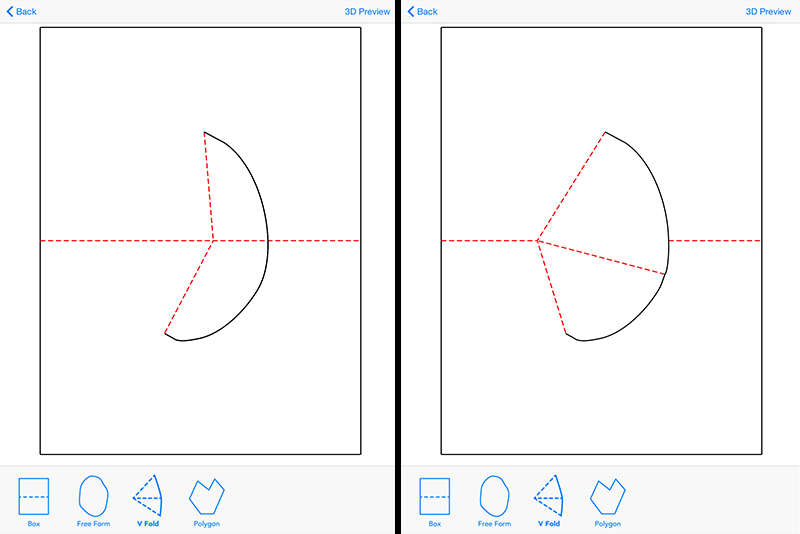
\includegraphics{figures/44_Tech_Validity/invalid_valid_vfold.png}
\caption{Left: an invalid, concave v-fold. Right: a valid, convex
v-fold.}
\end{figure}

\section{Constraints on Fold
Features}\label{constraints-on-fold-features}

Constraints are central to the implementation of Foldlings' algorithms,
which help our software provide an accurate preview of sketches, and
ensure that designs created with Foldlings will fold correctly. As an
educational tool, one of the primary benefits of our software might be
the development of an intuitive understanding of the limits of paper.

\subsection{Geometric Constraints}\label{geometric-constraints}

Several geometric constraints drive Foldling's algorithms. These
constraints are the core reason for the difficulty of creating designs
manually; a key advantage of our system is that these constraints are
resolved automatically.

\subsubsection{Box Fold}\label{box-fold}

\begin{figure}[htbp]
\centering
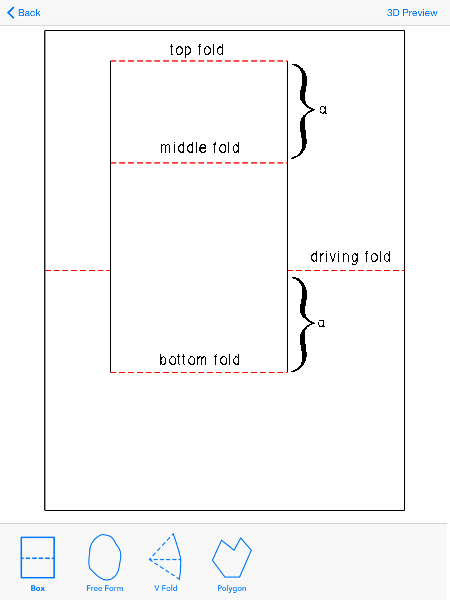
\includegraphics{figures/45_Tech_Constraints/boxfoldConstraints.pdf}
\caption{Geometric constraints for freeform features}
\end{figure}

A box fold is constrained by a relationship between its folds. Given a
top fold and bottom fold at fixed height, with a driving fold with a
height between the other two folds, the vertical distance between the
bottom fold and the driving fold must be equal to the distance between
the top fold and the middle fold of the feature.

This 90-degree angle constraint applies equally to freeform and polygon
features (at least, those that span a fold).

\subsubsection{Freeform}\label{freeform}

\begin{figure}[htbp]
\centering
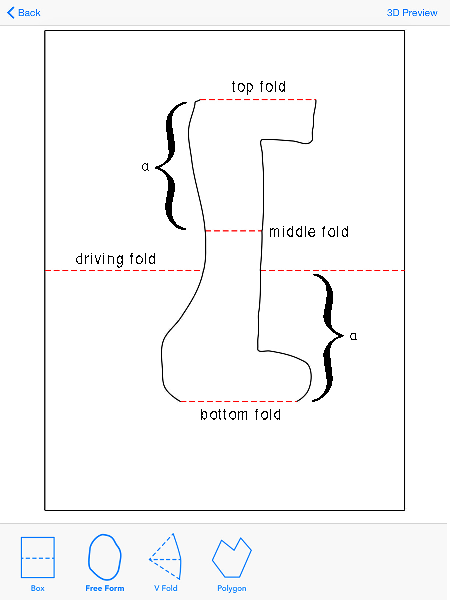
\includegraphics{figures/45_Tech_Constraints/freeformConstraints.pdf}
\caption{Geometric constraints for freeform features}
\end{figure}

Freeform fold heights are calculated similarly to those in a box fold.
After performing truncation\footnote{described
  \textbf{\textgreater{}\textgreater{}TODO: REF}} to place the top and
bottom folds of the freeform shape, we apply the 90-degree constraint to
place the middle fold in the feature. Of course, holes are not bound by
this constraint, because they do not have a driving fold.

As with all features, validity constraints are separate from geometric
constraints. Freeform shapes that intersect themselves do not have a
place for the middle fold, but by performing validity checks before
solving for geometric constraints, we avoid many problems and edge cases
that would otherwise occur.

\subsubsection{Polygon}\label{polygon}

\begin{figure}[htbp]
\centering
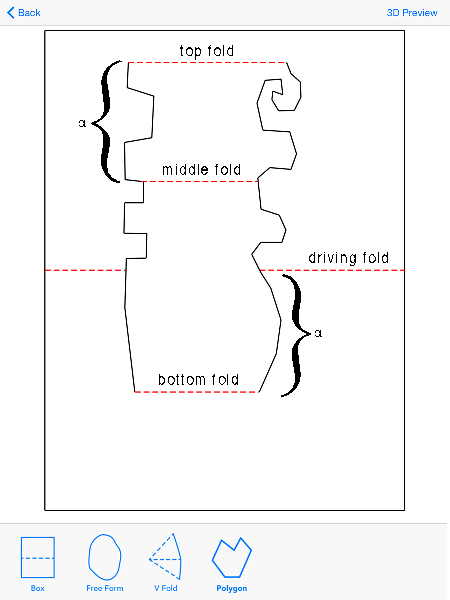
\includegraphics{figures/45_Tech_Constraints/polygonConstraints.pdf}
\caption{Geometric constraints for polygon features}
\end{figure}

The same constraints that apply to freeform shape apply to polygons.
Although the edges are constructed differently, polygons are essentially
a subset of freeform shapes, composed only of straight lines.

\subsubsection{V-Fold}\label{v-fold}

\begin{figure}[htbp]
\centering
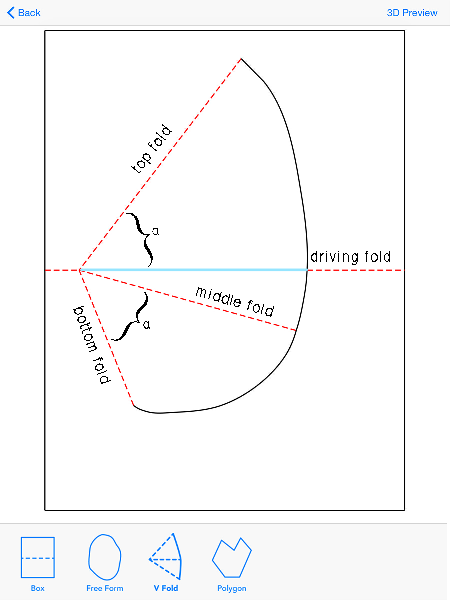
\includegraphics{figures/45_Tech_Constraints/vfoldConstraints.pdf}
\caption{Geometric constraints for freeform features}
\end{figure}

Although a v-fold also folds from zero to 180 degrees with the card, its
planes moves at non-orthogonal angles. The constraint on v-fold features
is therefore based on angle rather than height.

The simplest case of v-folds --- and the one most popularly constructed
by our user testers using manual methods --- is a symmetric v-fold. In
this case, the top and bottom angles of the fold are equal. The shape
approximates an isosceles triangle.

In the more complex case, the angles between the two diagonal folds and
the driving fold differ. Andrew Glassner demonstrates that for any
``single slit mechanism,'' the angle from the driving fold to either the
top or bottom fold must be equal to the angle between the opposite fold
and the middle fold (\citet{glassner1998interactive}, 3). This
constraint is only solvable if the sum of the angles between each
diagonal fold and driving fold is less than 180 degrees. Intuitively,
this constraint is not dissimilar from the constraint for box folds ---
the position of the middle fold is constrained by the driving fold's
relationship to the top and bottom folds.

\subsection{Physical Constraints}\label{physical-constraints}

In addition, the physicality of paper places constraints on where cuts
and folds can be placed. Depending on the manufacture method, there is
some minimum line length that can be cut or folded, and some minimum
distance folds and cuts must be apart. These depend on a number of
variables ranging from paper thickness to manufacture method (for
example, laser cutters have a higher tolerance for closely-drawn lines).
Even within a specific technology, there is also a wide variation in
cutting precision.

\begin{figure}[htbp]
\centering
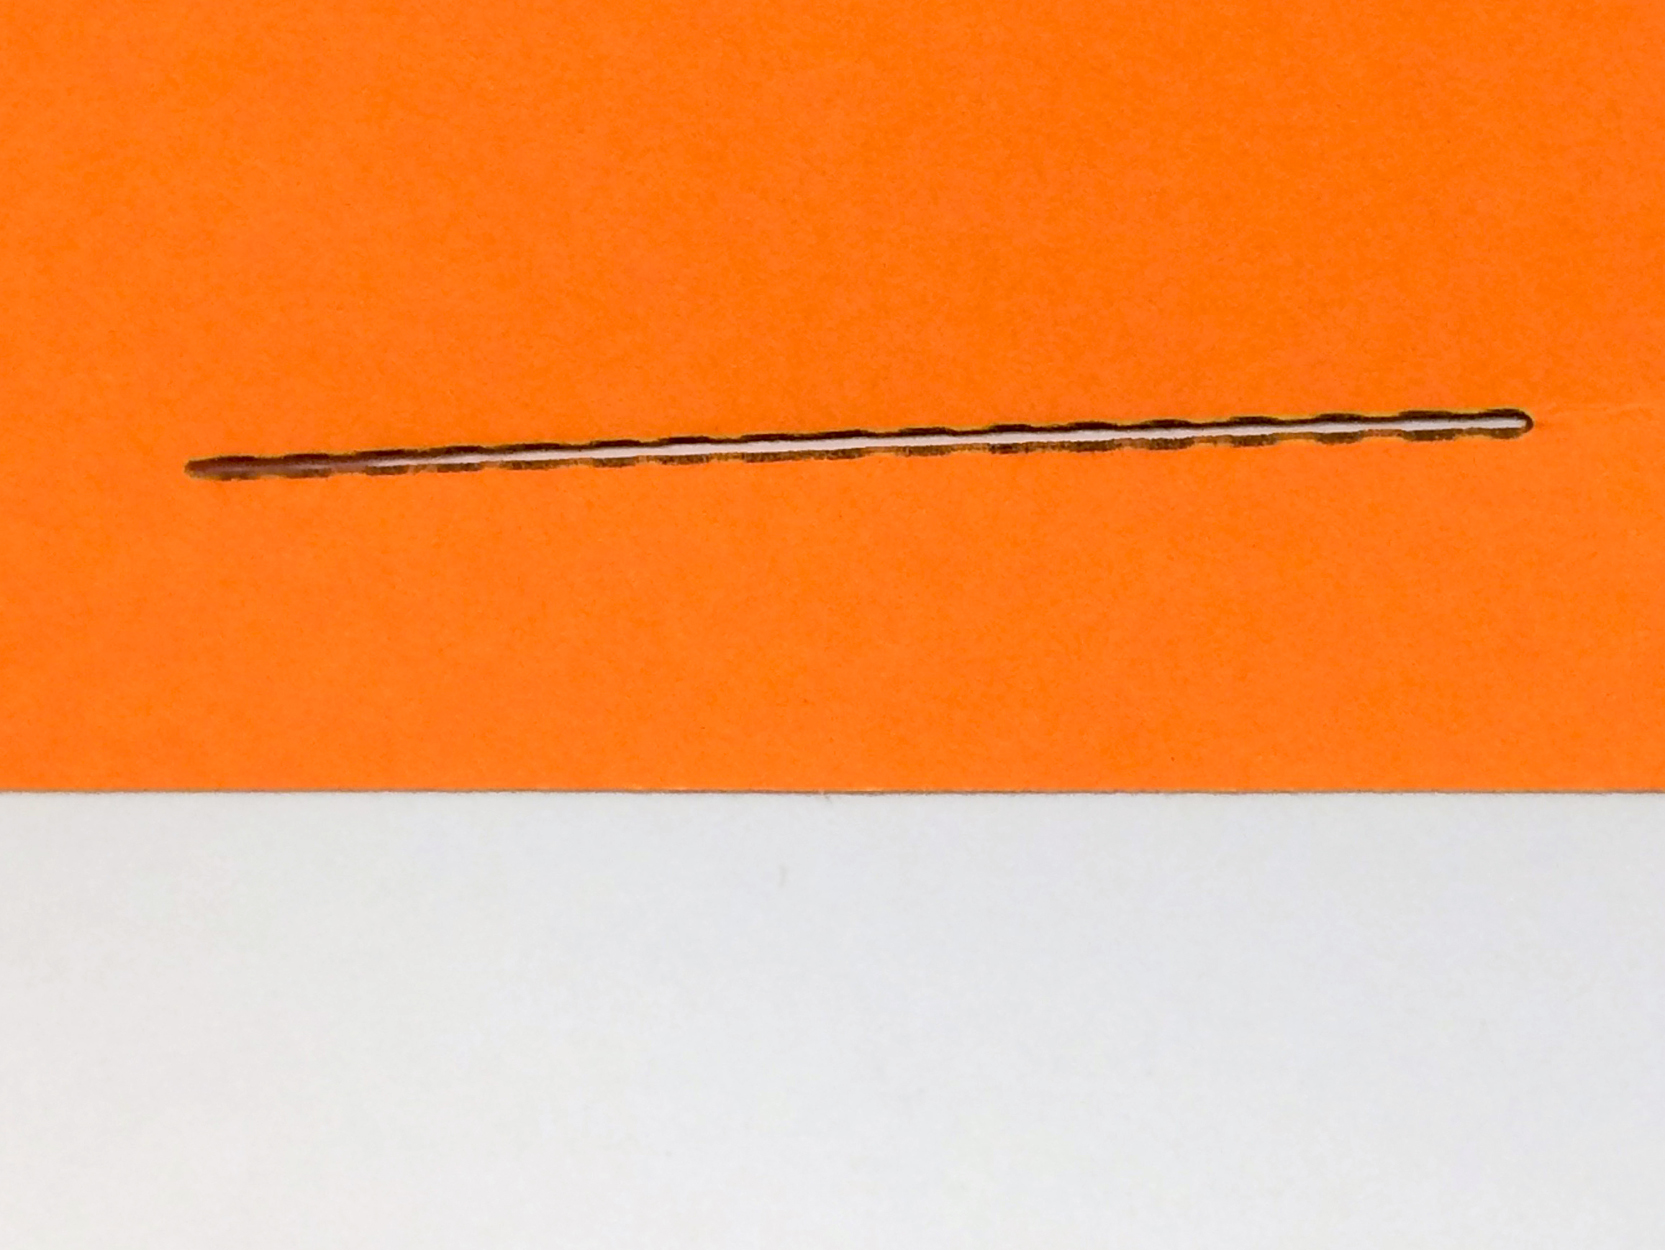
\includegraphics{figures/45_Tech_Constraints/tooclosecuts.jpg}
\caption{A malformed laser-cut fold. This is supposed to be a dotted
line, but because the dots were too close together, they have merged to
become a single cut.}
\end{figure}

In our software, we take this into account by incorporating a minimum
edge length constraint. The minimum edge length is the minimum length
for all edges in a feature. If the user creates a feature with edges
less than this length, a warning will appear as described in section
\textbf{\textgreater{}\textgreater{}TODO:CITE}, and the feature will not
be added to the sketch. This length constraint solves a variety of
potential problems: it prevents users from creating features that are
too small to tap, and insures that edges can be easily cut by hand or
using automated methods. We use the same length as the minimum edge
distance. In order to be valid, all edges in a feature must be at least
this distance from all other edges. In addition, we the line pattern for
folds in the SVG output to prevent the problem shown in figure
\textbf{\textgreater{}\textgreater{}TODO:CITE}. Because the fold line
pattern must be easy to crease while maintaining the card's integrity,
there is a tradeoff between ease of folding (dots close together) and
durability (dot further apart). We adjusted the line pattern to consist
of short dots spaced out slightly further than the minimum edge
distance. Although we discovered the line pattern through
experimentation, it performs well on multiple laser cutters, paper
types, and manual cutting. This pattern should work well for most common
paper cutting methods.

\chapter{User Studies}

While we performed frequent informal tests of our software with users,
these often consisted of a single user. The user tests described in this
chapter were larger-scale tests of key pieces of our software, and were
a major driving force in

\section{User Test at the Digital Arts
Exhibition}\label{user-test-at-the-digital-arts-exhibition}

\begin{figure}[htbp]
\centering
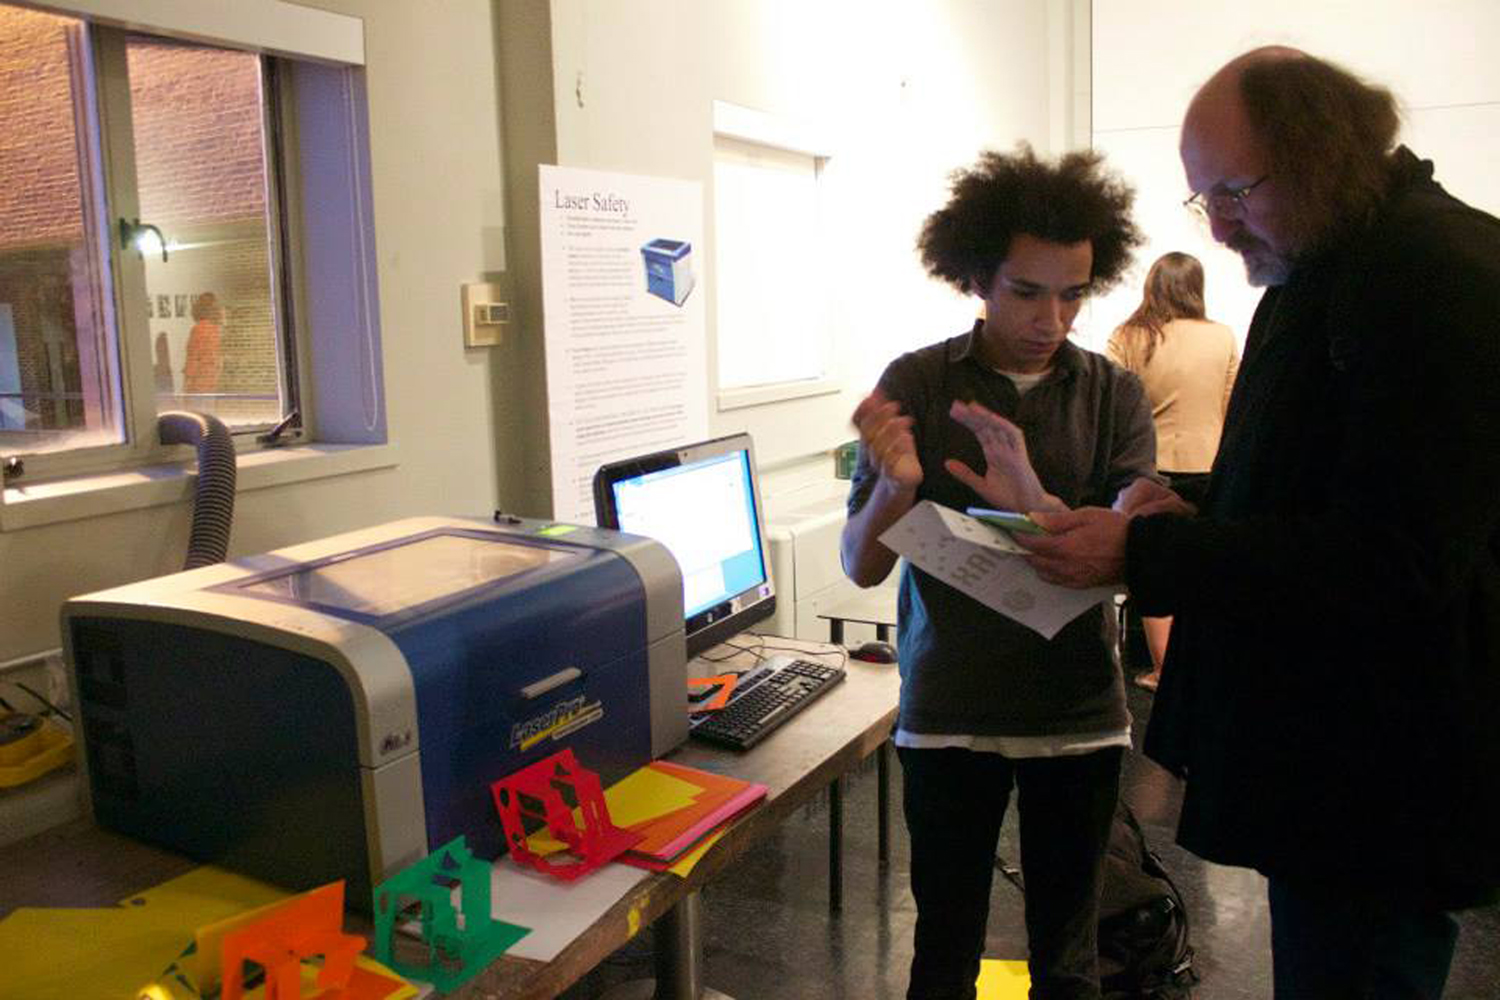
\includegraphics{figures/50_User_Study_Dax/dax_facebook_credit_Julietta_Gervase}
\caption{Foldlings at the Digital Arts Exhibition (\citet{daxphoto}).}
\end{figure}

On April 28, 2015, we tested our system with attendees of the Digital
Arts Exhibition at Dartmouth. After a brief demonstration of how to
create folds and preview their design, users designed cards using
Foldlings. Users drew sketches, and then sent an email containing an SVG
file to the computer connected to the laser cutter. Finally, they placed
a piece of paper in the laser cutter, and watched as the laser beam cut
out their design. Over the course of two hours, users cut and folded 31
popup cards.

The system we demonstrated at the exhibition was incomplete --- it
contained the basic box fold and freeform shape tools, but did not
include some advanced features of the final software, such as dragging
folds or shading based on plane orientation. The alpha software also
contained several bugs that disrupted the experience. However, the
system was usable enough for people to create cards, and observing user
behavior was invaluable in designing our final product.

Because users were new to our system --- and constrained by the pressure
of other users waiting to design cards --- designs were relatively
simple. Sketches generally contained between two and five fold features
in addition to the base card --- the most complex design contained ten
fold features. Despite their simplicity, sketches showed a wide range of
designs, ranging from abstract shapes to representational scenes ---
users sketched symbols, Chinese characters, and geometric forms. Most of
the sketches utilized both freeform and box fold features, mixing the
two element types to create a composition. One of the most popular
design elements was the user's name: 5 of the cards contained names or
initials. Roughly one third of the designs took advantage of nesting ---
constructing fold features inside each other.

Because users were able to quickly design and fabricate their design,
people generally left satisfied. People typically spent around 20
minutes at our booth, leaving with a popup card they had created.
However, the experience was not frictionless. Users were frustrated by
crashes: touching the screen with more than one finger or drawing while
calculating planes were the most common reasons for failure. Other
common complaints were the lack of a delete/undo button and that the UI
did not show which tool was currently selected.

Folding the fabricated design also presented difficulties. Although they
were able to see a 3D preview of their design while creating it, users
had often relinquished the iPad by the time they folded their design.
They were often unsure how to fold their card, and struggled to discover
the correct fold orientations. In some cases, it took longer for users
to fold their creation than to design it.

We observed several unexpected behaviors. A few users rotated the screen
to design a card in a landscape view, rather than the portrait
orientation implied by the orientation of the buttons and 3D preview.
They used this orientation to design cards that folded medially rather
than laterally. Several users also constructed overlapping features by
drawing on top of existing features. These features did not simulate
correctly, as they intersected with existing edges. However, this
behavior demonstrated a desire to construct more complex geometry. In
the final software we implement unions for fold features --- the most
recently-drawn feature occludes features underneath it, modifying their
edges.

Users also relied on the 3D preview to differing degrees. Some users
viewed the preview after every operation, while others only switched to
the preview occasionally. Many users relied on the 3D preview as a
reference to how to fold their popup card. We were surprised by this,
and conducted further user studies to determine the effectiveness of
methods of displaying 3D information.

\section{Visual Aids User Study}\label{visual-aids-user-study}

goal: test whether users understand the mapping of 2d fold patterns to
3d, and test the degree to which plane coloring, edge patterning, and a
3d preview help users understand how a popup card will fold.

Since. \textgreater{}\textgreater{}TODO: cite other research on visual
aids for folding slash other 2d to 3d vis

\subsection{Method}\label{method}

Each subject received a set of five laser cut cards, and we recorded the
time it takes them to successfully fold the card.

For each card, each subject was randomly given one of of the following
five aids:

\begin{enumerate}
\def\labelenumi{\arabic{enumi})}
\itemsep1pt\parskip0pt\parsep0pt
\item
  A two-dimensional design, showing planes shaded by whether they will
  be horizontal or vertical when folded.
\item
  A two-dimensional design, with edges patterned based on whether they
  are ``hills'' or ``valleys'' --- whether they fold towards or away
  from the card.
\item
  A video showing a simulation of the card folding in three dimensions.
\item
  A still image of the card folded in dimension.
\item
  No visual aid.
\end{enumerate}

The order of aids and cards was shuffled, and then balanced to ensure an
equal distribution of orderings. Eg. each visual aid has an equal chance
of being the first aid presented to a user and

Finally, we asked subjects to rank the visual aids

The effect each type of aid has on folding time will help determine
which types of visualization to include in Foldlings

\subsection{Results and Discussion}\label{results-and-discussion}

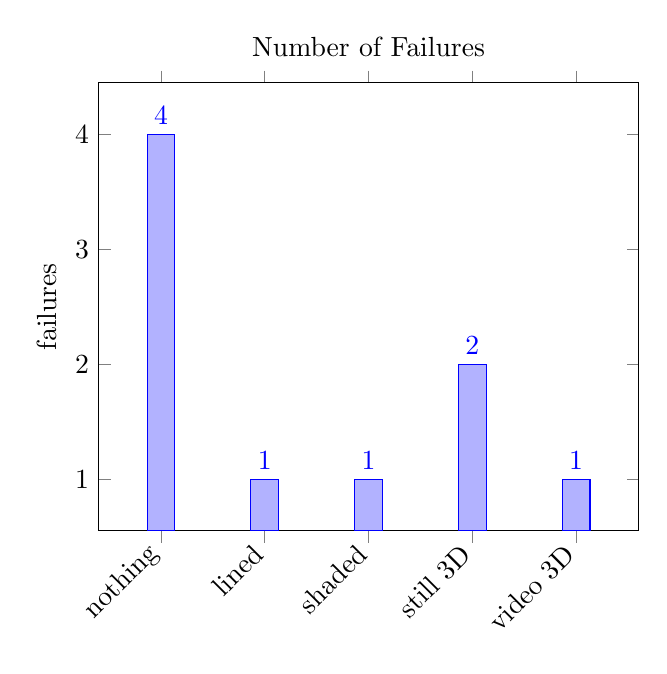
\begin{tikzpicture}
  \begin{axis}[
    title=Number of Failures,
    ybar,
    enlargelimits=0.15,
    legend style={at={(0.5,-0.2)},
      anchor=north,legend columns=-1},
    ylabel={failures},
    symbolic x coords={nothing,lined,shaded,still 3D,video 3D},
    xtick=data,
    nodes near coords, 
    nodes near coords align={vertical},
    x tick label style={rotate=45,anchor=east},
    ]
    \addplot coordinates {(nothing,4)(lined,1)(shaded,1)(still 3D,2)(video 3D,1)};
  \end{axis}
\end{tikzpicture}

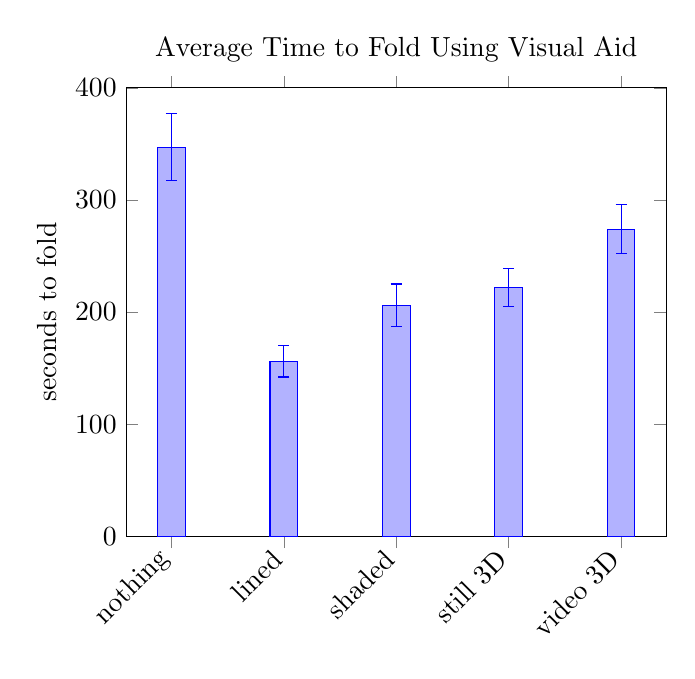
\begin{tikzpicture}
\begin{axis}[
  title=Average Time to Fold Using Visual Aid,
    ybar,
    ymin=0, ymax=400,
    legend style={at={(0.5,-0.2)},
     legend columns=-1},
    ylabel={seconds to fold},
    symbolic x coords={nothing,lined,shaded,still 3D,video 3D},
    xtick=data,
    x tick label style={rotate=45,anchor=east},
]
\addplot+[error bars/.cd,
y dir=both,y explicit]
coordinates {
    (nothing,347) +- (0.0, 30)
    (lined,156) +- (0.0, 14)
    (shaded,206) +- (0.0, 19)
    (still 3D,222) +- (0.0, 17)
    (video 3D,274) +- (0.0, 22)};
\end{axis}
\end{tikzpicture}

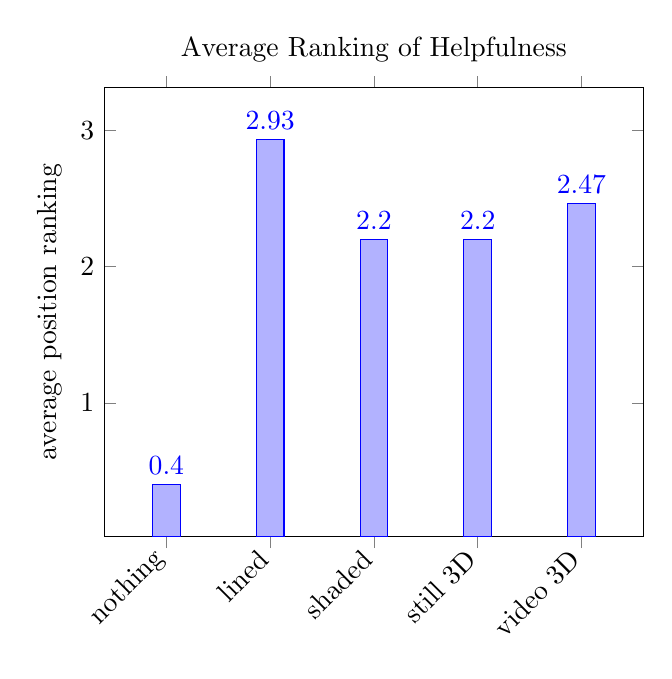
\begin{tikzpicture}
  \begin{axis}[
    title=Average Ranking of Helpfulness,
    ybar,
    enlargelimits=0.15,
    legend style={at={(0.5,-0.2)},
      anchor=north,legend columns=-1},
    ylabel={average position ranking},
    symbolic x coords={nothing,lined,shaded,still 3D,video 3D},
    xtick=data,
    nodes near coords, 
    nodes near coords align={vertical},
    x tick label style={rotate=45,anchor=east},
    ]
    \addplot coordinates {(nothing,0.4)(lined,2.933333333)(shaded,2.2)(still 3D,2.2)(video 3D,2.466666667)};
  \end{axis}
\end{tikzpicture}

\section{Final User Study}\label{final-user-study}

As a final test of software, we compared the usability with Foldlings to
traditional manual popup design methods. First, we presented
participants with a completed popup card, and asked them to replicate
the design using manual cutting and folding and to create the design
using our software. The order was randomized, so half of participants
were given were given the manual first, and half started with Foldlings.
We timed how long the participants took to complete the design. Next, we
gave users a free-form design exercise. Finally, we asked participants
to rate the experience of using our tool and their satisfaction with the
popup card they produced.

We are still collecting results from the study, which will be presented
at our thesis presentation on August 25th, 2015.

\chapter{Conclusions}

We plan to release Foldlings in the Apple App Store in September. In
many ways, the primary test of our software will be the extent to which
real users are able to achieve their design goals. However, we can make
several conclusions about the success of our tool. In general, users
find the process of designing popup cards more intuitive with the
current version of Foldlings than with previous versions of our software
or manual methods. Additionally, we have qualitative evidence that
suggest that users can create a wide range of complex cards, faster and
with more precision than using manual methods. That said, there is much
work to be done on this and related popup-card design problems.

\section{User Interface Future Work}\label{user-interface-future-work}

\subsection{Modifications to the Master
Card}\label{modifications-to-the-master-card}

Currently, our software only allows for one size and type of master card
feature. That is, a greeting-card sized piece of paper, with a single
driving fold in the center. Allowing modifications to the driving fold
might allow users to change paper size, rotate the card so that the
middle fold is vertical, or construct a diagonal fold for the master
card.

\subsection{Multiple Cards}\label{multiple-cards}

Currently, our software simulates cuts and folds performed on a single
piece of paper. In order to support combinations of interlocking
sketches, we would need to create an interface that allow for connecting
pop-up card elements in 3D. Although very complex to implement, this
interface could ultimately allow for a far more complex arrangement of
features that our software currently affords (\citet{hart2007modular}).

\subsection{Safe Area Guides}\label{safe-area-guides}

Often, users wish construct a fully-contained popup card. That is, a
card that can close fully, with no portions of internal fold features
visible when the card is closed. In order to achieve this design in a
symmetrical card, all features with a driving fold must be created such
that their planes will not extend beyond the bound of the master card
when fully folded. We could add ``safe area'' guides and warnings to
indicate this area to users that want to add that additional constraint
to their design.

\section{Algorithms \& Implementation Future
Work}\label{algorithms-implementation-future-work}

\subsection{Feature Intersections}\label{feature-intersections}

Feature intersections are only partially implemented, and do not always
succeed. To fully-implement feature intersections, we would need to
refactor our FoldFeature class to add feature intersections a primary
component. This would replace the current method of intersecting
features with folds --- \emph{splitFoldByOcclusion} --- and would allow
for more generalizable intersections between features.

\subsection{Concurrency}\label{concurrency}

A key limitation of Foldlings is that all functions currently run on a
single thread. As a consequence, the user is sometimes blocked by
operations that could be performed in the background. For example, when
completing a feature, out app ignores touch input until the feature is
added to the sketch and planes are calculated. This can cause a slight
but noticeable delay between actions. Restructuring our algorithms to
perform computationally-heavy operations in the background would reduce
lag between actions, allowing users to design more quickly and fluidly.

\section{Potential Applications}\label{potential-applications}

\emph{This section is co-authored with Marissa Allen}
\textbf{\textgreater{}\textgreater{}TODO: get comments/more content from
marissa}

As a general-purpose design tool for cuts and folds, Foldlings has a
wide variety of potential applications. For example, Melina Blees et al
present a graphene transistor that is constructed through kirigami
methods \citet{blees2014graphene}. Simple, usable interfaces for
designing complex kirigami structures are needed to advance similar
research.

One exciting application of Foldlings is as a tool for developing
advanced spatial reasoning skills. Taylor et al present a curriculum
that uses popup card design as a tool for building mathematics and
spatial reasoning skills \citet{taylor2013think3d}
\citet{olson_mathematics_2004}. A tool like Foldlings would likely
increase the effectiveness of such a program, since much of the
experimentation could happen more quickly in software than using manual
methods. Because our code is open source, advanced students could even
modify our software to develop new fold features and interactions.

\chapter{Appendix}

\captionsetup[figure]{list=no}

\section{Appendix A: User Interface
Mockups}\label{appendix-a-user-interface-mockups}

Mockups

\section{Appendix B: Designs Created at
DAX}\label{appendix-b-designs-created-at-dax}

Mockups

\section{Appendix C: Visual Aids User Study
Materials}\label{appendix-c-visual-aids-user-study-materials}

\subsection{Lined Visual Aids}\label{lined-visual-aids}

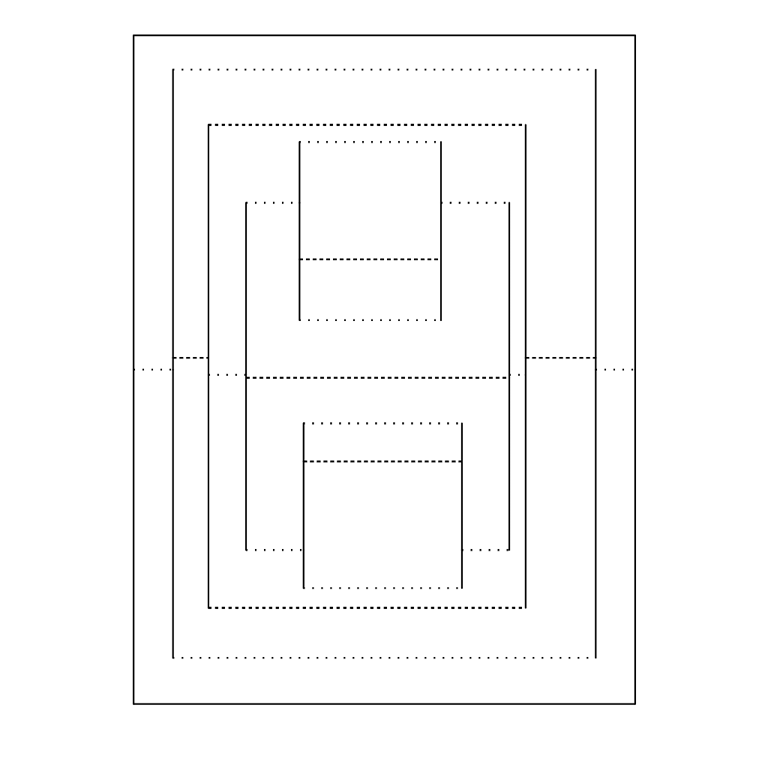
\includegraphics{figures/92_Appendix_Visual_Aids_Materials/lined_card1.png}\\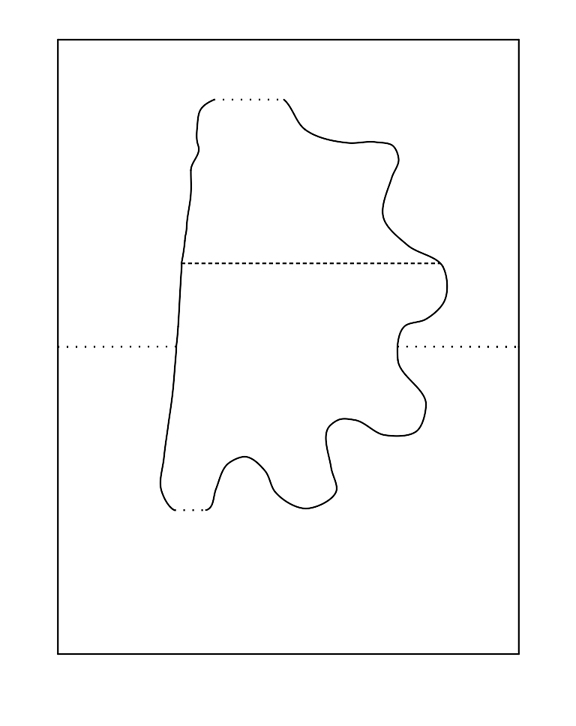
\includegraphics{figures/92_Appendix_Visual_Aids_Materials/lined_card2.png}\\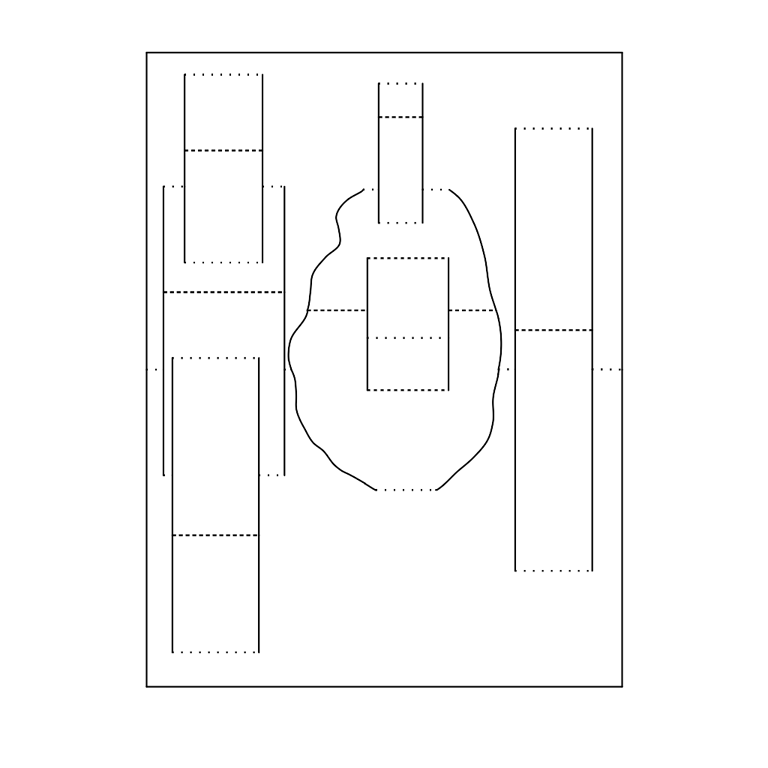
\includegraphics{figures/92_Appendix_Visual_Aids_Materials/lined_card3.png}\\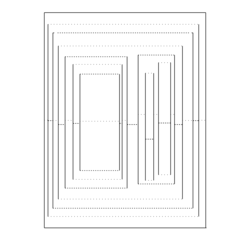
\includegraphics{figures/92_Appendix_Visual_Aids_Materials/lined_card4.png}\\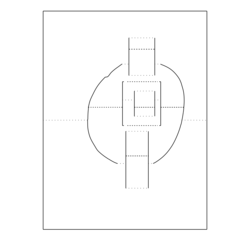
\includegraphics{figures/92_Appendix_Visual_Aids_Materials/lined_card5.png}\\
\#\#Shaded Visual Aids

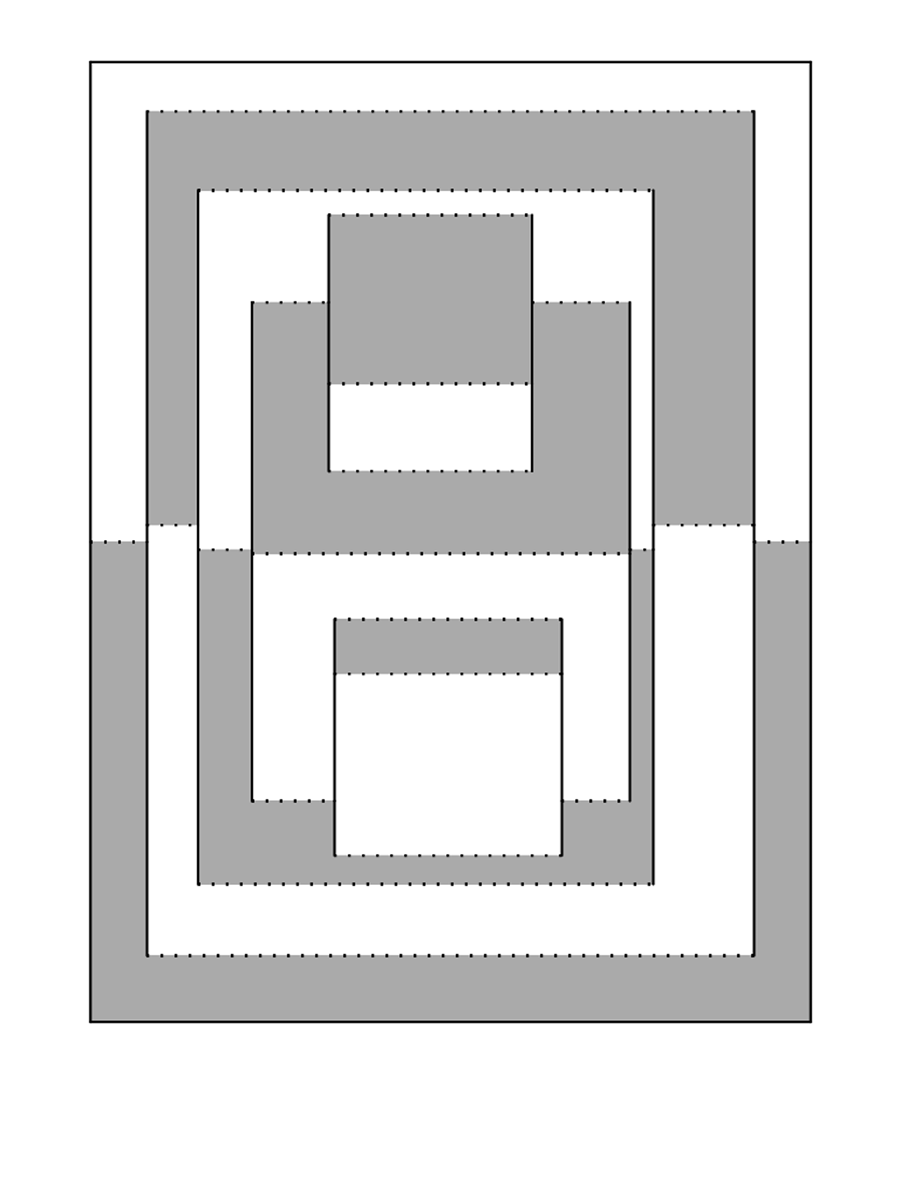
\includegraphics{figures/92_Appendix_Visual_Aids_Materials/shaded_card1.png}\\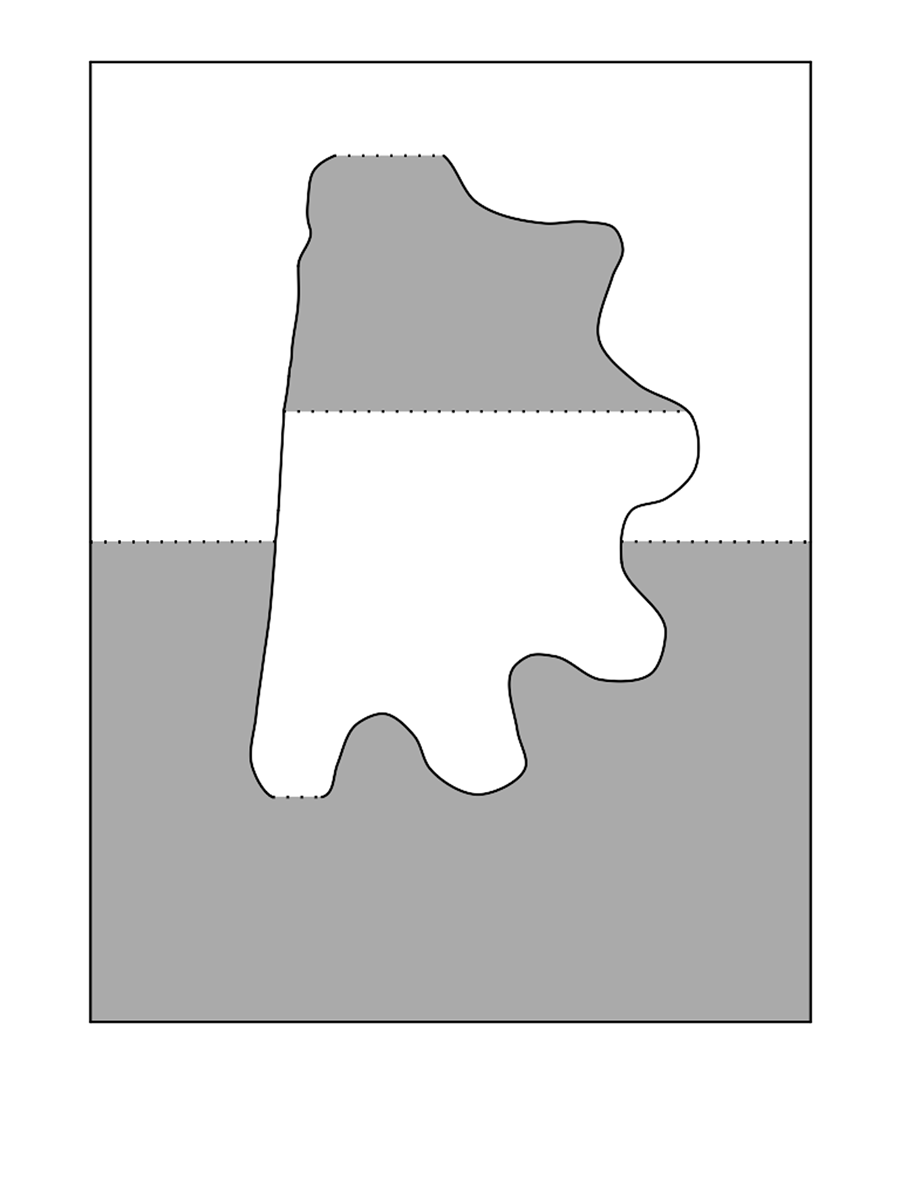
\includegraphics{figures/92_Appendix_Visual_Aids_Materials/shaded_card2.png}\\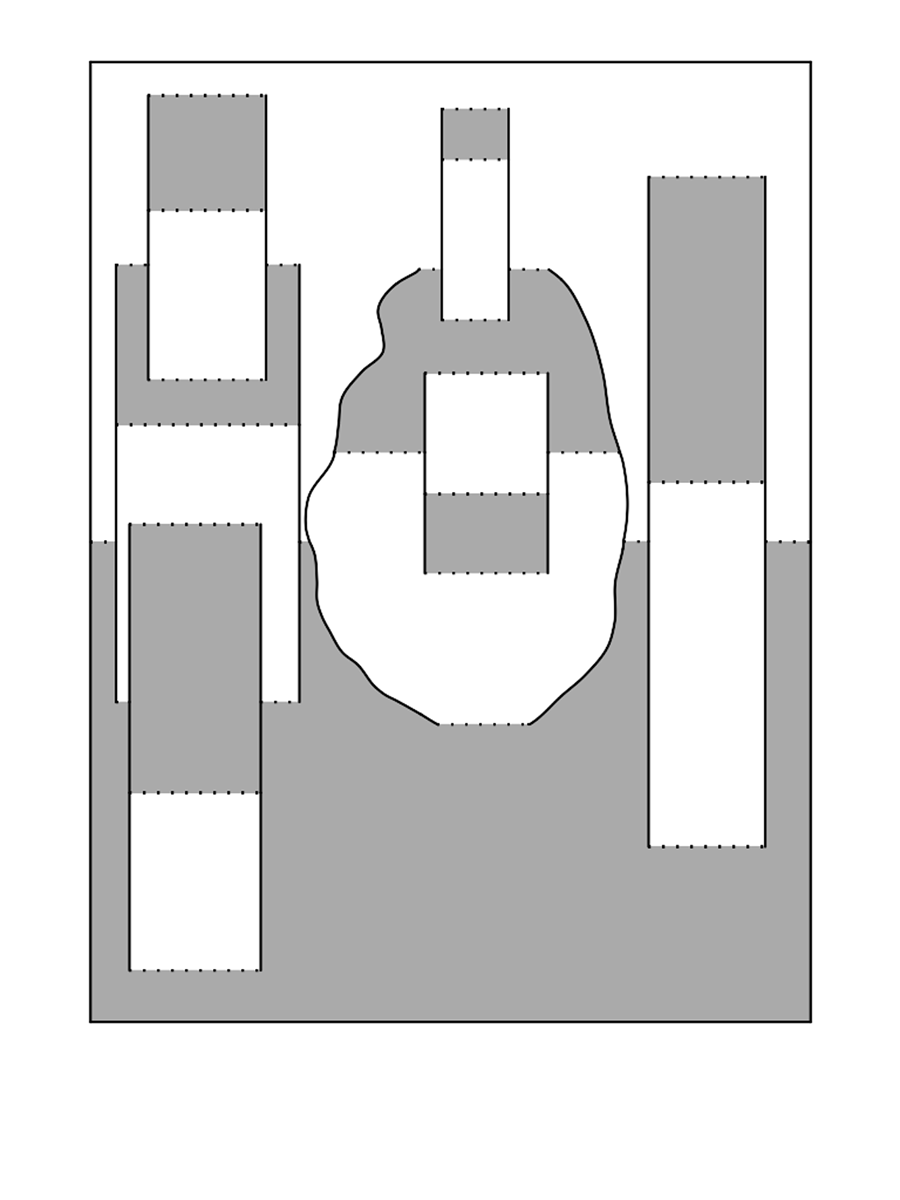
\includegraphics{figures/92_Appendix_Visual_Aids_Materials/shaded_card3.png}\\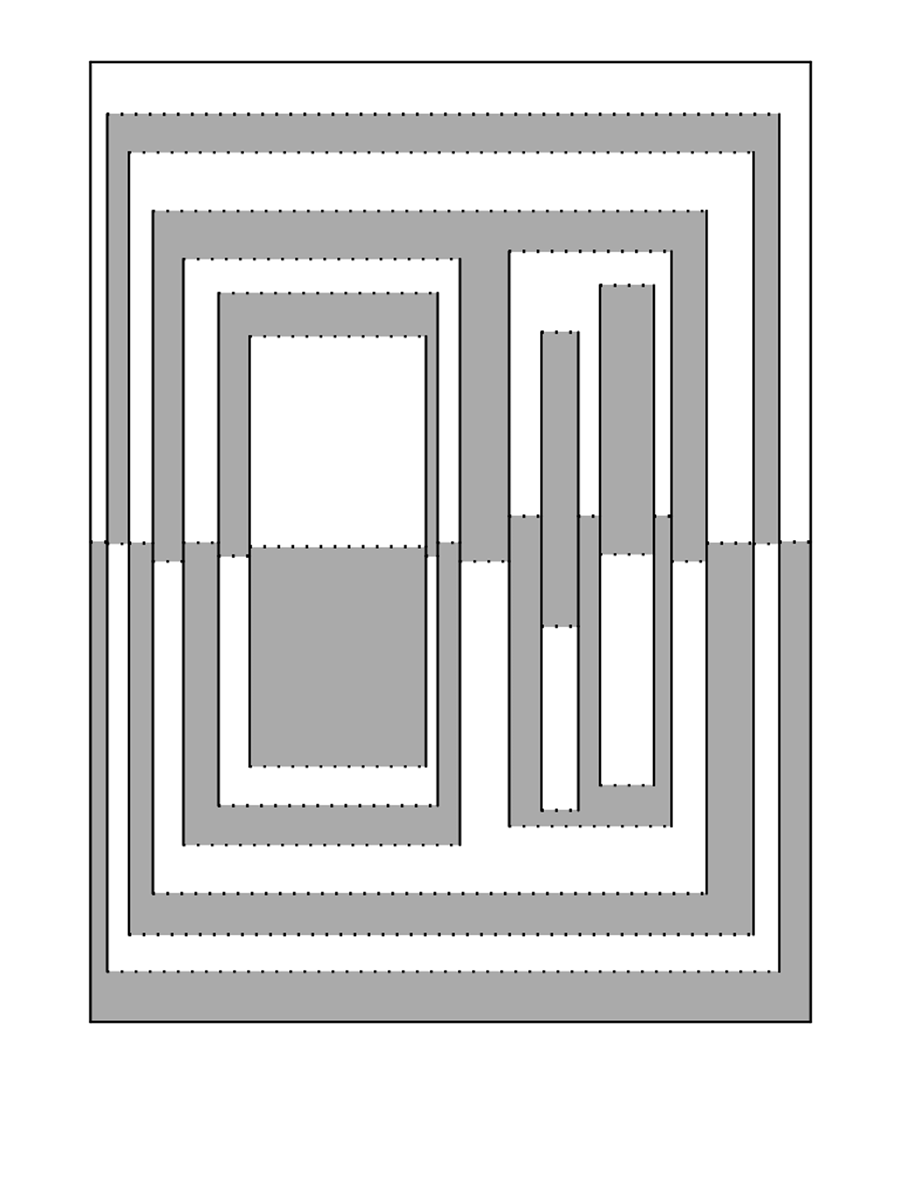
\includegraphics{figures/92_Appendix_Visual_Aids_Materials/shaded_card4.png}\\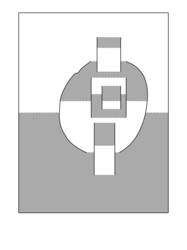
\includegraphics{figures/92_Appendix_Visual_Aids_Materials/shaded_card5.png}\\
\#\#Still 3D Visual Aids

\textbf{\textgreater{}\textgreater{}TODO FIX FORMATTING}

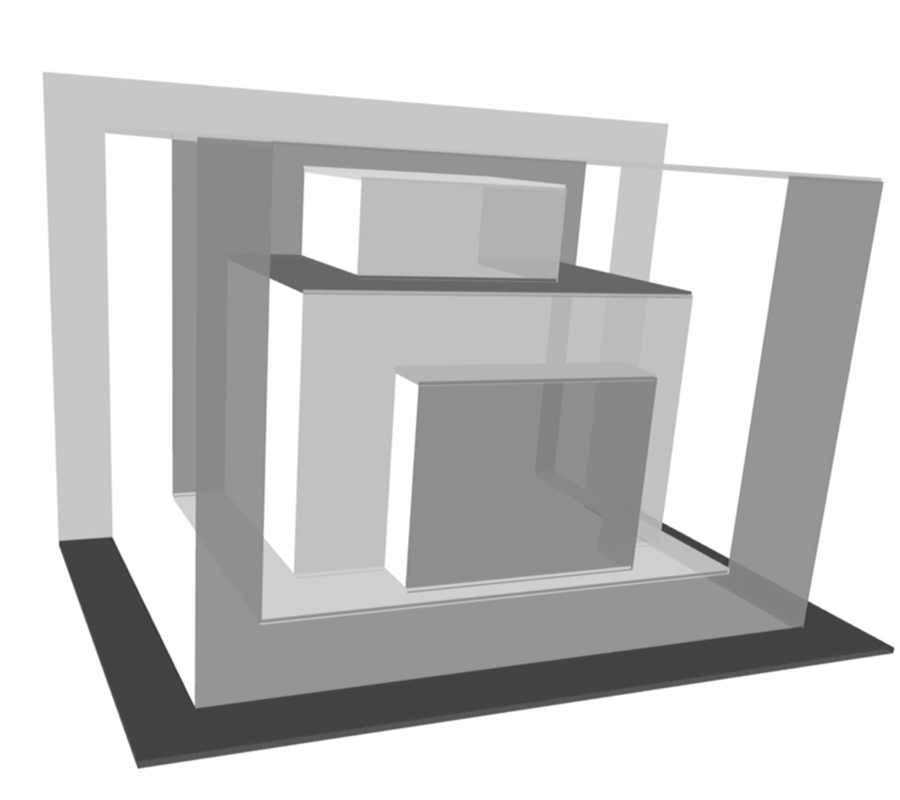
\includegraphics{figures/92_Appendix_Visual_Aids_Materials/still_card1.png}\\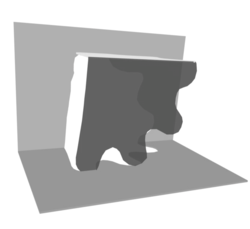
\includegraphics{figures/92_Appendix_Visual_Aids_Materials/still_card2.png}\\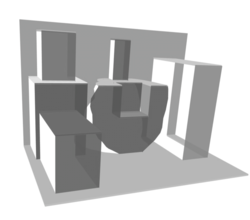
\includegraphics{figures/92_Appendix_Visual_Aids_Materials/still_card3.png}\\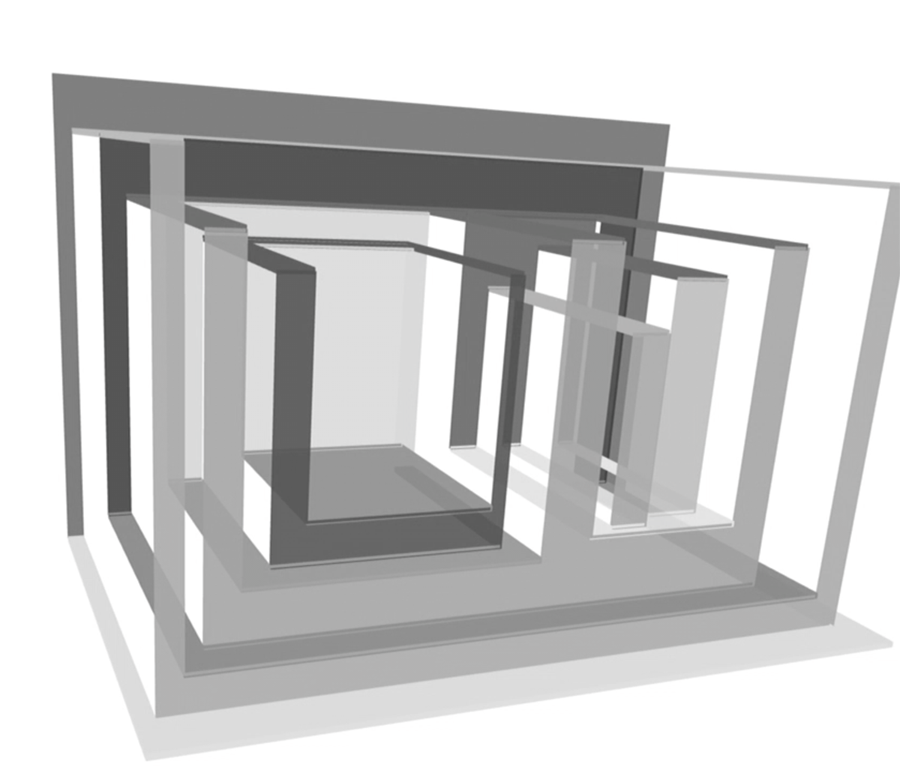
\includegraphics{figures/92_Appendix_Visual_Aids_Materials/still_card4.png}\\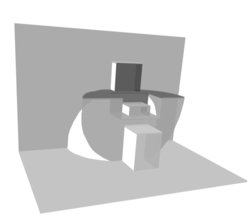
\includegraphics{figures/92_Appendix_Visual_Aids_Materials/still_card5.png}\\
\#\#Video Visual Aids

Note: these were displayed on a laptop screen as a video; only
screenshots are shown here.

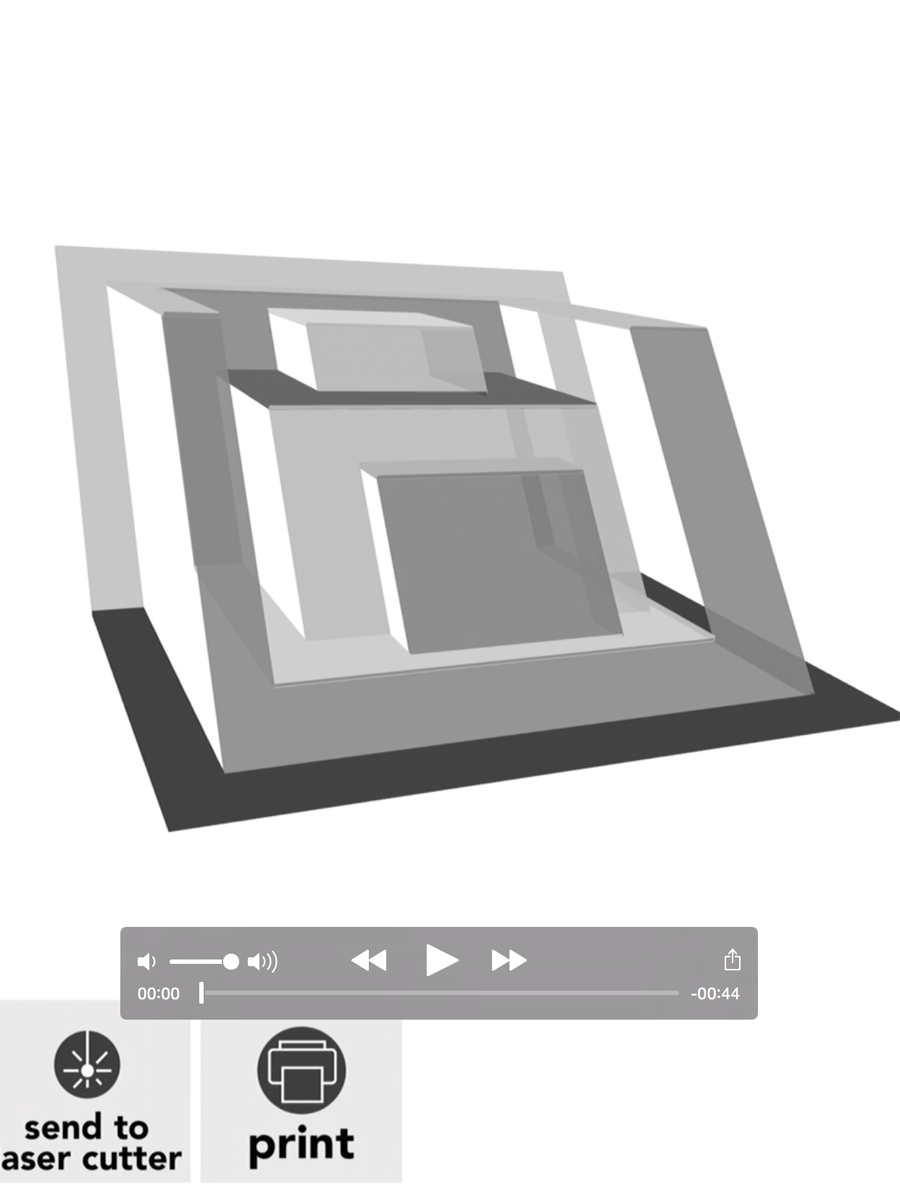
\includegraphics{figures/92_Appendix_Visual_Aids_Materials/video_card1.png}\\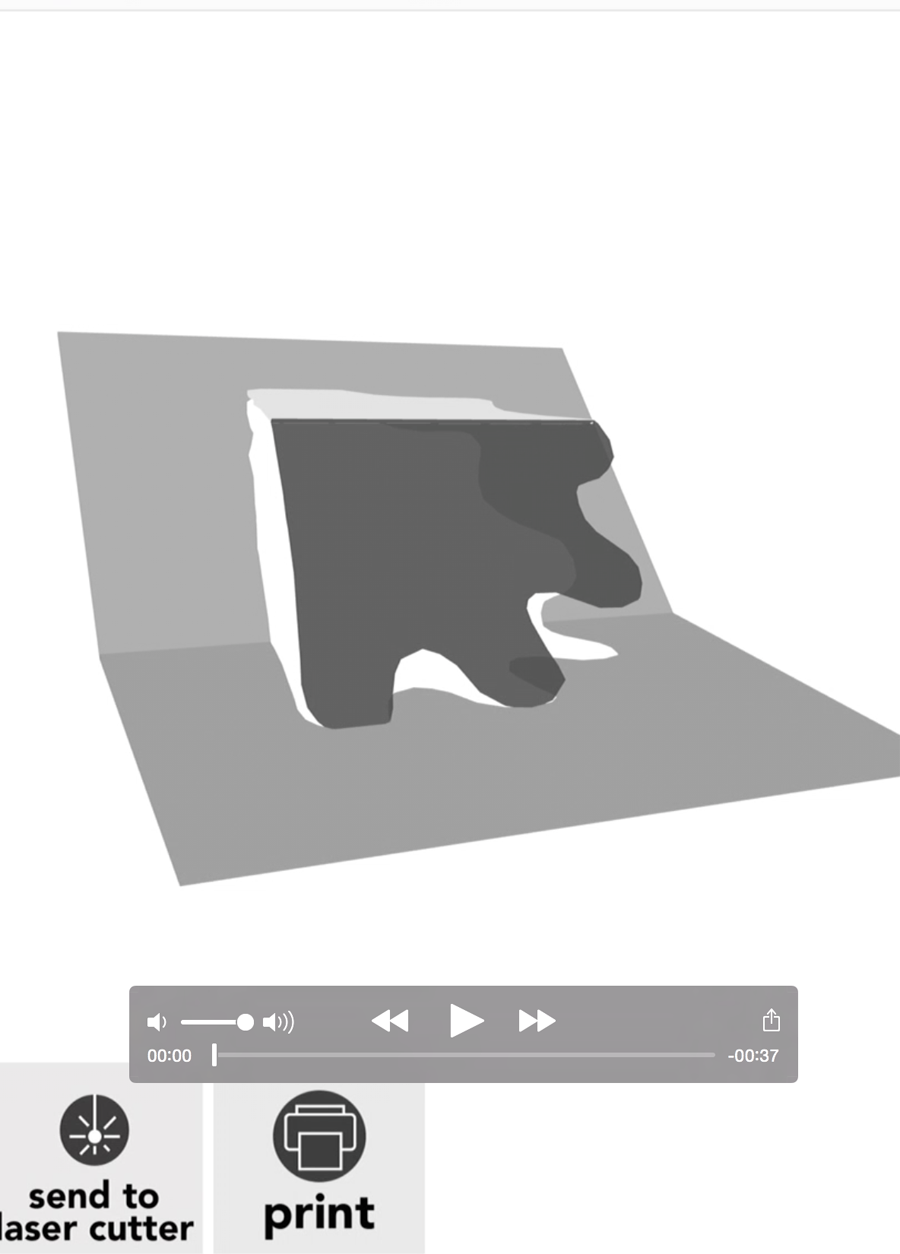
\includegraphics{figures/92_Appendix_Visual_Aids_Materials/video_card2.png}\\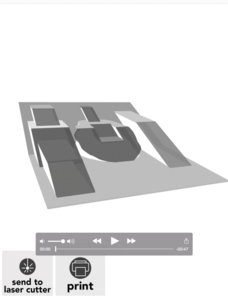
\includegraphics{figures/92_Appendix_Visual_Aids_Materials/video_card3.png}\\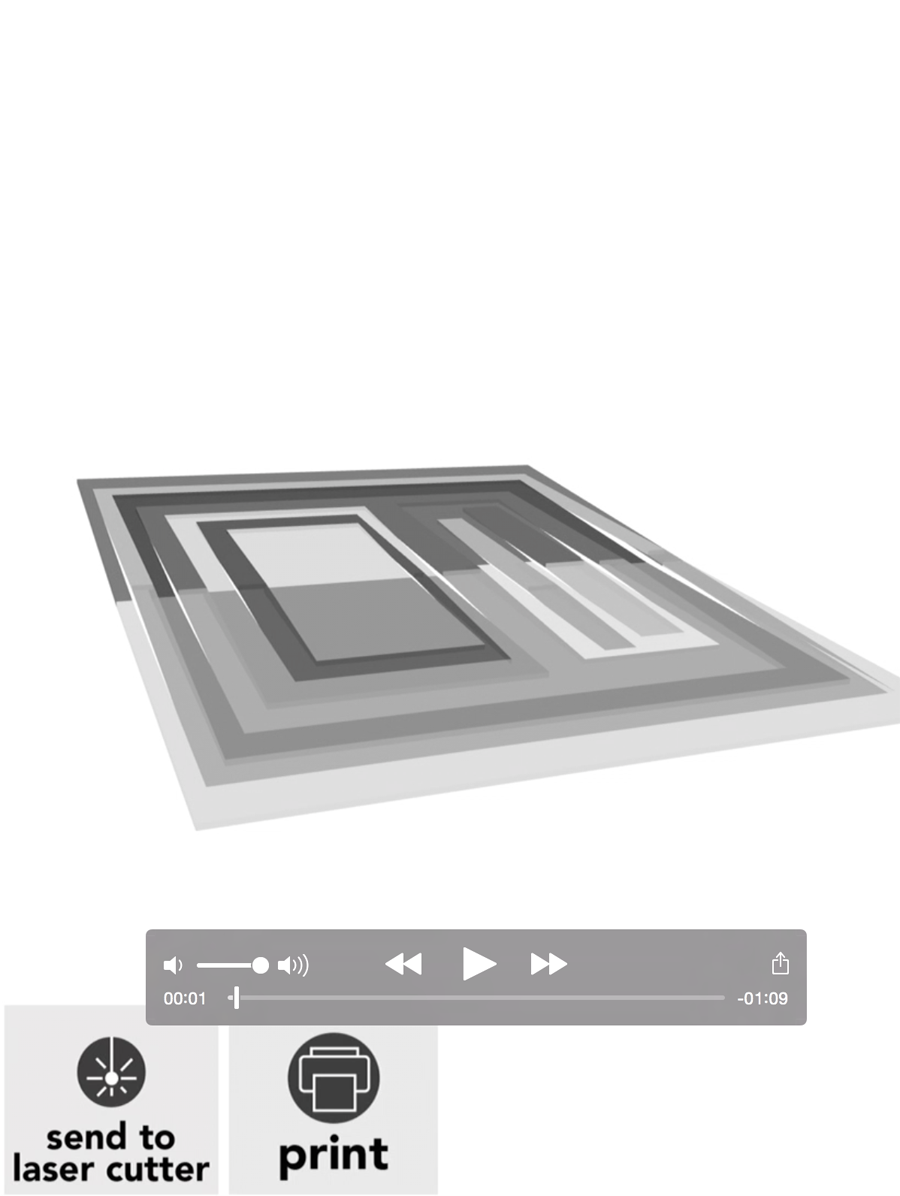
\includegraphics{figures/92_Appendix_Visual_Aids_Materials/video_card4.png}\\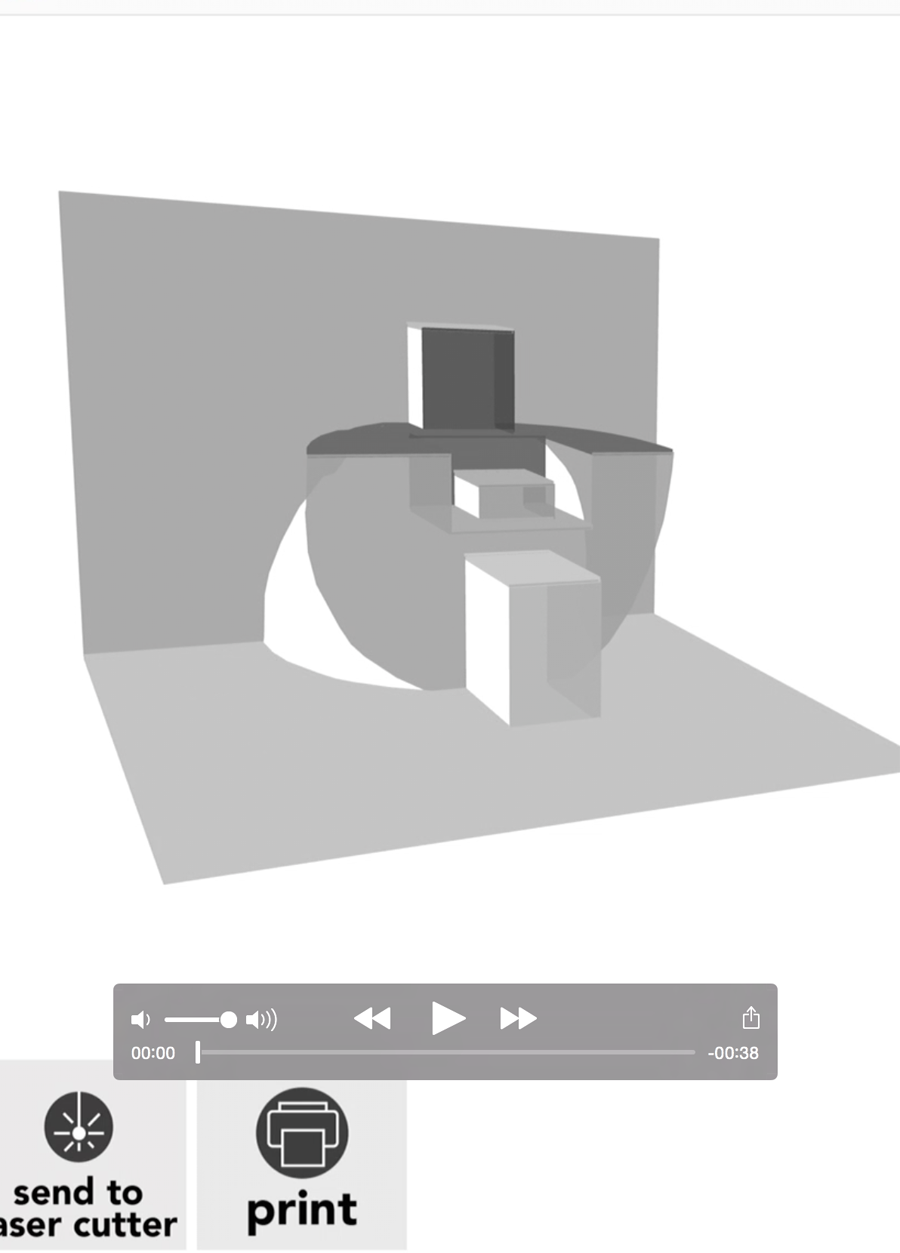
\includegraphics{figures/92_Appendix_Visual_Aids_Materials/video_card5.png}\\
\#\#Completed Cards

\includegraphics{figures/92_Appendix_Visual_Aids_Materials/completed_card1.png}\\\includegraphics{figures/92_Appendix_Visual_Aids_Materials/completed_card2.png}\\\includegraphics{figures/92_Appendix_Visual_Aids_Materials/completed_card3.png}\\\includegraphics{figures/92_Appendix_Visual_Aids_Materials/completed_card4.png}\\\includegraphics{figures/92_Appendix_Visual_Aids_Materials/completed_card5.png}\\

\section{Appendix D: Sample Cards}\label{appendix-d-sample-cards}

This appendix contains examples of cards designed using our software and
manufactured by hand.

\begin{figure}[htbp]
\centering
\includegraphics{figures/93_Appendix_Sample_Cards/bday_combined.pdf}
\caption{}
\end{figure}

\begin{figure}[htbp]
\centering
\includegraphics{figures/93_Appendix_Sample_Cards/city_combined.pdf}
\caption{}
\end{figure}

\begin{figure}[htbp]
\centering
\includegraphics{figures/93_Appendix_Sample_Cards/floral_combined.pdf}
\caption{}
\end{figure}

\begin{figure}[htbp]
\centering
\includegraphics{figures/93_Appendix_Sample_Cards/forest_combined.pdf}
\caption{}
\end{figure}

\begin{figure}[htbp]
\centering
\includegraphics{figures/93_Appendix_Sample_Cards/love_combined.pdf}
\caption{}
\end{figure}

\begin{figure}[htbp]
\centering
\includegraphics{figures/93_Appendix_Sample_Cards/sine_combined.pdf}
\caption{}
\end{figure}

\section{Appendix D: Separation of
Work}\label{appendix-d-separation-of-work}

I collaborated on this project with Marissa Allen. Although we worked
collaboratively on the software, each of us presents an individual
thesis paper. Our responsibilities on the software were as follows: Nook
concentrated on tools and interactions, including performing user
studies and processing user input, while Marissa concentrated on 3D
interactions and data structures, including the algorithms for shading
and traversing planes.

%END_INCLUDES

% \appendix
% 

\section*{Appendix A: User Study 1}
\addcontentsline{toc}{section}{Appendix A: User Study 1}

% \begin{figure}[h!]
% \begin{center}$
% \begin{array}{c c}
% \includegraphics[width=2.3in]{figures/exp1/test-01.png} &
% \includegraphics[width=2.3in]{figures/exp1/test-02.png} \\ 
% \includegraphics[width=2.3in]{figures/exp1/test-03.png} &
% \includegraphics[width=2.3in]{figures/exp1/test-04.png} \\ 
% \includegraphics[width=2.3in]{figures/exp1/test-05.png} &
% \includegraphics[width=2.3in]{figures/exp1/test-06.png} \\ 
% \includegraphics[width=2.3in]{figures/exp1/test-07.png} &
% \includegraphics[width=2.3in]{figures/exp1/test-08.png} \\ 
% \includegraphics[width=2.3in]{figures/exp1/test-09.png} &
% \includegraphics[width=2.3in]{figures/exp1/test-10.png}
% \end{array}$
% \end{center}
% \end{figure}

% \begin{figure}[h]
% \begin{center}$
% \begin{array}{c c}
% \includegraphics[width=2.5in]{figures/exp1/test-11.png} &
% \includegraphics[width=2.5in]{figures/exp1/test-12.png} \\ 
% \includegraphics[width=2.5in]{figures/exp1/test-13.png} &
% \includegraphics[width=2.5in]{figures/exp1/test-14.png} \\ 
% \includegraphics[width=2.5in]{figures/exp1/test-15.png} &
% \includegraphics[width=2.5in]{figures/exp1/test-16.png} \\ 
% \includegraphics[width=2.5in]{figures/exp1/test-17.png} &
% \includegraphics[width=2.5in]{figures/exp1/test-18.png} \\ 
% \includegraphics[width=2.5in]{figures/exp1/test-19.png} &
% \includegraphics[width=2.5in]{figures/exp1/test-20.png}
% \end{array}$
% \end{center}
% \caption{Trial images from User Study 2, ctd.}
% \end{figure}
% 


\section*{Appendix B: User Study 2}
\addcontentsline{toc}{section}{Appendix B: User Study 2}

% Confidence interval:
%   The mean of	none minus greens equals -0.418776725758
%   95% confidence interval of this difference: From -0.822466706937 to -0.015086744578 
% Intermediate values used in calculations:
%   t = 2.2602
%   df = 12

% \begin{table}[h!]
% \centering
%  \begin{tabular}{|m{5em} || m{6em} | m{10em} | m{10em}|} 
%  \hline
%  Group & Affect & Adjectives & Next Day Plans \\ 
%  \hline\hline
%  none & 0.0516810976 & "boodle boodle" & "poodle doodles" \\ 
%  none & 0.636986 & "devious" & "chomp will eat the other fish" \\
%  greens & 0.8030303 & "adorable, heartwarming, calming, Nemo-like, colorful, whimsical" & "ill be another shark stereotype misunderstanding that is also resolved" \\
%  greens & 0.720838249 & "Active, Outgoing, Determined" & "He will make more friends" \\
%  greens & 0.7200083 & "nervous, eager, determined. lonely, friendly, motivated, unrelenting" & "ill have a picnic/lunch party (something where they all eat together)." \\
%  none & 0.74491477 & "timid, lonely, scared, shy, cautious, unsure" & "thing new and make even more friends. probubly go on an adventure " \\
%  none & 0.5 & "Friendly" & "he will make a new friend " \\
%  none & 0.0566625558 & "Naive, friendly, innocent, slow" & "They will have to hunt for food / eat things" \\
%  none & 0 & "Smiley, Nice, Hungry" & "Chomp's going to eat more fish." \\
%  greens & 0.9906599 & "sad, lonely, misunderstood, nice, friendly" & "Chomps will have a better day with his new sea friends" \\
%  none & 0.156289 & "Shy, ruthless, deceptive" & "Chomp will eat more of his classmates" \\
%  none & 0.5 & "Friendly" & "He struggles with his natural hunting instincts" \\
%  none & 0.114778049 & "accidental fish eater" & "i think he's going to eat more fish by accident" \\
%  none & 0.0525114536 & "crafty" & "Chomp will eat more of the "children"" \\
%  none & 0.807181537 & "Friendly, shy, and loyal" & "more friends and enjoy Ms Pufferfish's lesson plan, no matter what it is. \\ [1ex] 
%  \hline
%  \end{tabular}
% \end{table}


% \begin{figure}[h]
% \begin{center}$
% \begin{array}{c c}
% \includegraphics[width=2.5in]{figures/exp2_screencaps/01.png} &
% \includegraphics[width=2.5in]{figures/exp2_screencaps/02.png} \\ 
% \includegraphics[width=2.5in]{figures/exp2_screencaps/03.png} &
% \includegraphics[width=2.5in]{figures/exp2_screencaps/04.png} \\ 
% \includegraphics[width=2.5in]{figures/exp2_screencaps/05.png} &
% \includegraphics[width=2.5in]{figures/exp2_screencaps/06.png} \\ 
% \includegraphics[width=2.5in]{figures/exp2_screencaps/07.png} &
% \includegraphics[width=2.5in]{figures/exp2_screencaps/08.png} \\ 
% \includegraphics[width=2.5in]{figures/exp2_screencaps/09.png} &
% \includegraphics[width=2.5in]{figures/exp2_screencaps/10.png}
% \end{array}$
% \end{center}
% \caption{Trial images from User Study 2}
% \end{figure}

% \begin{figure}[h]
% \begin{center}$
% \begin{array}{c c}
% \includegraphics[width=2.5in]{figures/exp2_screencaps/11.png} &
% \includegraphics[width=2.5in]{figures/exp2_screencaps/11_alt.png} \\ 
% \includegraphics[width=2.5in]{figures/exp2_screencaps/12.png} &
% \includegraphics[width=2.5in]{figures/exp2_screencaps/13.png} \\ 
% \includegraphics[width=2.5in]{figures/exp2_screencaps/13_alt.png} &
% \includegraphics[width=2.5in]{figures/exp2_screencaps/14.png} \\ 
% \includegraphics[width=2.5in]{figures/exp2_screencaps/15.png} &
% \includegraphics[width=2.5in]{figures/exp2_screencaps/16.png} \\ 
% \includegraphics[width=2.5in]{figures/exp2_screencaps/17.png} &
% \includegraphics[width=2.5in]{figures/exp2_screencaps/18.png}
% \end{array}$
% \end{center}
% \caption{Trial images from User Study 2, ctd.}
% \end{figure}






% 

\section*{Appendix C: Distribution of Work}
\addcontentsline{toc}{section}{Appendix C: Distribution of Work}

% As part of the requirement for a joint thesis this sections identifies the different work performed by each of the two authors. 

% Rukmini Goswami took the lead on:
% \begin{itemize}
%  \setlength\itemsep{-0.5em}
%  \item user study design and process
%  \item analysis of results
%  \item experimental setup in Unity3D
%  \item EyeTribe initial experimentation
%  \item statistical methods
%  \item all artwork for the future work
% \end{itemize}

% Tim Tregubov took the lead on: 
% \begin{itemize}
%  \setlength\itemsep{-0.5em}
%  \item scaffolding out the Unity3D C\# classes and framework. 
%  \item designing the narrative framework structure
%  \item Tobii SDK integration
%  \item gaze and fixation data processing
%  \item stack architecture and code structure
% %  \begin{itemize}
% %     \setlength\itemsep{-0.5em}
% %     \item for thi
% %  \end{itemize}
% \end{itemize}

 
% \section*{Appendix D: Preview images from FrameShift the novel}
\addcontentsline{toc}{section}{Appendix D: Preview images from FrameShift — the novel}
% \begin{figure}[h!]
% \begin{center}$
% \begin{array}{c c}
% \includegraphics[width=2.3in]{figures/appendixD/01.png} &
% \includegraphics[width=2.3in]{figures/appendixD/02.png} \\ 
% \includegraphics[width=2.3in]{figures/appendixD/03.png} &
% \includegraphics[width=2.3in]{figures/appendixD/04.png} \\ 
% \includegraphics[width=2.3in]{figures/appendixD/05.png} &
% \includegraphics[width=2.3in]{figures/appendixD/06.png} \\ 
% \includegraphics[width=2.3in]{figures/appendixD/07.png} &
% \includegraphics[width=2.3in]{figures/appendixD/08.png} \\ 
% \includegraphics[width=2.3in]{figures/appendixD/09.png} &
% \includegraphics[width=2.3in]{figures/appendixD/10.png}
% \end{array}$
% \end{center}
% \end{figure}

\singlespacing

\bibliography{nook_citations}
\addcontentsline{toc}{chapter}{Bibliography}



\end{document}
